% ~~~~~~~~~~~~ %
% tab size = 4 %
% ~~~~~~~~~~~~ %

% WARNING: if the compiler returns the error ``incompatible list can't be unboxed''
% try to decomment the following \RequirePackage command:
%\RequirePackage{atbegshi} 

\documentclass % ~~~~~~~~~~~~~~~~~~~~~~~~~~~~~~~~~~~~~~~~~~~~~~~~~~ %
[																	%
	aspectratio=1610,                                               %
	11pt,															%
	hyperref={pdfpagelabels=false},									%
	xcolor	= pdftex, dvipsnames, table,							%
% 	handout,														% decomment for handouts
]																	%
{beamer}															%
%																	%
\usepackage[latin1]{inputenc}										%
\usepackage[english]{babel}											%
\usepackage{type1cm}												%
\usepackage{type1ec}												%
\usepackage[T1]{fontenc}											%
\usepackage{lmodern}												%
\usepackage{amsmath, amssymb, amsfonts, amsthm}						%
\usepackage{graphicx}												%
\usepackage{hyperref}												%
\usepackage{booktabs}												%
\usepackage{bm}														%
\usepackage{tikz}		                                            %
                                                                    %
\setbeamerfont{note page}{size=\large}                              %
%                                                                   %
% \usetikzlibrary{arrows,decorations.text,decorations.pathmorphing}	%
% \usetikzlibrary{decorations.footprints,fadings,calc,trees,mindmap}%
% \usetikzlibrary{shadows,patterns,positioning,shapes,matrix,fit}	%
% \usetikzlibrary{intersections,datavisualization,plotmarks,spy}	%
\usepackage{pgfplots}												%
% \pgfplotsset{compat=1.3}											%
%\usetikzlibrary{external}											%
%\tikzexternalize[shell escape=-enable-write18]						%
%																	%
\usepackage{pgfpages}												%
\setbeamercovered{invisible}
\setbeameroption{show notes on second screen=left}					% comment for just 1 screen
%																	%
% ~~~~~~~~~~~~~~~~~~~~~~~~~~~~~~~~~~~~~~~~~~~~~~~~~~~~~~~~~~~~~~~~~ %
%																	%
\def\DarkBlue		{black!70!blue}%{black!40!blue}					%
\def\DarkGray		{black!70!white}								%
\def\DarkGreen		{black!40!green}								%
\def\DarkRed		{black!40!red}									%
\def\DarkYellow		{black!40!yellow}								%
\def\DarkOrange		{black!40!orange}								%
%																	%
\def\Blue			{black!30!blue}									%
\def\Gray			{black!50!white}								%
\def\Green			{black!10!green}								%
\def\Red			{black!10!red}									%
\def\Yellow			{black!10!yellow}								%
\def\Orange			{black!10!orange}								%
%																	%
\def\LightBlue		{white!40!blue}									%
\def\LightGray		{white!92!black}%{white!70!white}				%
\def\LightGreen		{white!40!green}%{white!40!green}				%
\def\LightRed		{white!40!red}									%
\def\LightYellow	{white!40!yellow}								%
\def\LightOrange	{white!40!orange}								%
%																	%
% ~~~~~~~~~~~~~~~~~~~~~~~~~~~~~~~~~~~~~~~~~~~~~~~~~~~~~~~~~~~~~~~~~ %
%																	%
\def\Background		{white}%{\pgfsetfillopacity{.95}}%{white}		%
\def\Foreground		{\DarkBlue}%{black}								%
\def\Primary		{\Blue}%{\Blue}									%
\def\Secondary		{\LightGray}%{\Gray}							%
%																	%
\def\StrongPrimary	{\Primary!80!black}								%
\def\SoftPrimary	{\Primary!20!white}								%
\def\StrongSecondary{\Secondary!80!black}							%
\def\SoftSecondary	{\Secondary!20!white}							%
%																	%
% ~~~~~~~~~~~~~~~~~~~~~~~~~~~~~~~~~~~~~~~~~~~~~~~~~~~~~~~~~~~~~~~~~ %
%																	%
\graphicspath{{./Images/}}											%
%																	%

\pgfdeclarelayer{ultrabackground}
\pgfdeclarelayer{background}
\pgfdeclarelayer{foreground}
\pgfsetlayers{ultrabackground,background,main,foreground}


\newcommand{\JustPrimary}		[1]{\textcolor{\StrongPrimary}{#1}}
\newcommand{\ItPrimary}			[1]{\textcolor{\StrongPrimary}{\textit{#1}}}
\newcommand{\BoldPrimary}		[1]{\textcolor{\StrongPrimary}{\textbf{#1}}}
\newcommand{\BoldItPrimary}		[1]{\textcolor{\StrongPrimary}{\textit{ \textbf{#1} }}}
\newcommand{\ItBoldPrimary}		[1]{\BoldItPrimary{#1}}
%
\newcommand{\JustSecondary}		[1]{\textcolor{\StrongSecondary}{#1}}
\newcommand{\ItSecondary}		[1]{\textcolor{\StrongSecondary}{\textit{#1}}}
\newcommand{\BoldSecondary}		[1]{\textcolor{\StrongSecondary}{\textbf{#1}}}
\newcommand{\BoldItSecondary}	[1]{\textcolor{\StrongSecondary}{\textit{ \textbf{#1} }}}
\newcommand{\ItBoldSecondary}	[1]{\BoldItSecondary{#1}}



\newcommand {\PrimaryRectangle} [1]
{
	\begin{center}
	\begin{tikzpicture}
		%
		\node
		[
			shape			= rectangle,		% shape
			rounded corners	= 0.2cm,			% shape
			minimum width	= 0.7cm,			%
			minimum height	= 0.7cm,			%
			line width		= 0cm,				% thickness of the border
			fill			= \SoftPrimary,		%
			draw			= \StrongPrimary,	% draw the border with this color
			line width		= 0.1cm,			% thickness
			text width		= 0.8\textwidth,	% max. width of the text
			align			= center,			% text alignment
			inner xsep		= 0.2cm,			%
			inner ysep		= 0.2cm,			%
		]
		{#1};
		%
	\end{tikzpicture}
	\end{center}
}


\newcommand {\SecondaryRectangle} [1]
{
	\begin{center}
	\begin{tikzpicture}
		%
		\node
		[
			shape			= rectangle,		% shape
			rounded corners	= 0.2cm,			% shape
			minimum width	= 0.7cm,			%
			minimum height	= 0.7cm,			%
			line width		= 0cm,				% thickness of the border
			fill			= \SoftSecondary,	%
			draw			= \StrongSecondary,	% draw the border with this color
			line width		= 0.1cm,			% thickness
			text width		= 0.8\textwidth,	% max. width of the text
			align			= center,			% text alignment
			inner xsep		= 0.2cm,			%
			inner ysep		= 0.2cm,			%
		]
		{#1};
		%
	\end{tikzpicture}
	\end{center}
}


\newcommand {\PrimaryRectangleWithCaption} [3]
{
	\begin{center}
	\begin{tikzpicture}
		%
		\node (a)
		[
			shape			= rectangle,		% shape
			rounded corners	= 0.2cm,			% shape
			minimum width	= 0.7cm,			%
			minimum height	= 0.7cm,			%
			fill			= \SoftPrimary,		%
			draw			= \StrongPrimary,	% draw the border with this color
			line width		= 0.1cm,			% thickness
			text width		= 0.8\textwidth,	% max. width of the text
			align			= center,			% text alignment
			inner xsep		= 0.3cm,			%
			inner ysep		= 0.3cm,			%
		]
		{#2};
		%
		\node
		[
			shape			= rectangle,		% shape
			rounded corners	= 0.2cm,			% shape
			anchor			= mid,
			fill			= \SoftPrimary,		%
			draw			= \StrongPrimary,	% draw the border with this color
			text			= \StrongPrimary,	%
			align			= center,			% text alignment
			line width		= 0.1cm,			% thickness
			inner xsep		= 0.2cm,			%
			inner ysep		= 0.2cm,			%
		]
		at (a.#3)
		{#1};
		%
	\end{tikzpicture}
	\end{center}
}


\newcommand {\SecondaryRectangleWithCaption} [3]
{
	\begin{center}
	\begin{tikzpicture}
		%
		\node (a)
		[
			shape			= rectangle,		% shape
			rounded corners	= 0.2cm,			% shape
			minimum width	= 0.7cm,			%
			minimum height	= 0.7cm,			%
			fill			= \SoftSecondary,	%
			draw			= \StrongSecondary,	% draw the border with this color
			line width		= 0.1cm,			% thickness
			text width		= 0.8\textwidth,	% max. width of the text
			align			= center,			% text alignment
			inner xsep		= 0.3cm,			%
			inner ysep		= 0.3cm,			%
		]
		{#2};
		%
		\node
		[
			shape			= rectangle,		% shape
			rounded corners	= 0.2cm,			% shape
			anchor			= mid,
			fill			= \SoftSecondary,	%
			draw			= \StrongSecondary,	% draw the border with this color
			text			= \StrongSecondary,	%
			align			= center,			% text alignment
			line width		= 0.1cm,			% thickness
			inner xsep		= 0.2cm,			%
			inner ysep		= 0.2cm,			%
		]
		at (a.#3)
		{#1};
		%
	\end{tikzpicture}
	\end{center}
}




% ~~~~~~~~~~~~~~~~~~~~~~~~~~~~~~~~~~~~~~~~~~~~~~~~~~~~~~~~~~~~~ %
\newcommand{\EstimatedSignal}						[0]	{\widehat{\Signal}}
\newcommand{\OptimallyEstimatedSignal}				[0]	{\widehat{\Signal}^{*}}
\newcommand{\OptimallyBayesEstimatedSignal}			[0]	{\widehat{\Signal}^{*}_{\text{Bayes}}}
\newcommand{\OptimallyCostFunctionEstimatedSignal}	[0]	{\widehat{\Signal}^{*}_{\text{c.f.}}}
%
\newcommand{\EstimatedSignalAt}						[1]	{\EstimatedSignal \left( #1 \right)}
\newcommand{\OptimallyEstimatedSignalAt}			[1]	{\OptimallyEstimatedSignal \left( #1 \right)}
\newcommand{\OptimallyBayesEstimatedSignalAt}		[1]	{\OptimallyBayesEstimatedSignal \left( #1 \right)}
\newcommand{\OptimallyCostFunctionEstimatedSignalAt}[1]	{\OptimallyCostFunctionEstimatedSignal \left( #1 \right)}
%
\newcommand{\EstimatedSignalAtSet}						[1]	{\EstimatedSignal_{#1}}
\newcommand{\OptimallyEstimatedSignalAtSet}				[1]	{\OptimallyEstimatedSignal_{#1}}
\newcommand{\OptimallyBayesEstimatedSignalAtSet}		[1]	{\OptimallyBayesEstimatedSignal_{#1}}
\newcommand{\OptimallyCostFunctionEstimatedSignalAtSet}	[1]	{\OptimallyCostFunctionEstimatedSignal_{#1}}




\newcommand{\EstimatedEigenfunctionWeight}			[1]
			{\widehat{a}_{#1}}
\newcommand{\SetOfEstimatedEigenfunctionsWeights}	[0]
			{\widehat{\SetOfEigenfunctionsWeights}}
\newcommand{\EigenfunctionsWeightsEstimationError}	[0]
			{\widetilde{\SetOfEigenfunctionsWeights}}




\newcommand{\EstimatedEigenfunctionWeightOfSensor}			[2]
			{\widehat{a}_{#1, #2}}
\newcommand{\SetOfEstimatedEigenfunctionsWeightsOfSensor}	[1]
			{\widehat{\SetOfEigenfunctionsWeights}_{#1}}
\newcommand{\EigenfunctionsWeightsEstimationErrorOfSensor}	[1]
			{\widetilde{\SetOfEigenfunctionsWeights}_{#1}}
\newcommand{\LocallyEstimatedEigenfunctionWeightOfSensor}	[2]
			{\widehat{a}_{#1, #2}^{loc}}




\newcommand{\SetOfLocallyEstimatedEigenfunctionsWeights}				[0]
			{\widehat{\SetOfEigenfunctionsWeights}^{\text{loc}}}
\newcommand{\SetOfLocallyEstimatedEigenfunctionsWeightsOfSensor}		[1]
			{\widehat{\SetOfEigenfunctionsWeights}^{\text{loc}}_{#1}}
\newcommand{\SetOfLocallyBayesEstimatedEigenfunctionsWeights}			[0]
			{\widehat{\SetOfEigenfunctionsWeights}_{\text{Bayes}}^{\text{loc}}}
\newcommand{\SetOfLocallyCostFunctionEstimatedEigenfunctionsWeights}	[0]
			{\widehat{\SetOfEigenfunctionsWeights}_{\text{c.f.}}^{\text{loc}}}
%
\newcommand{\SetOfLocallyBayesEstimatedEigenfunctionsWeightsOfSensor}			[1]
			{\widehat{\SetOfEigenfunctionsWeights}_{\text{Bayes}, #1}^{\text{loc}}}
\newcommand{\SetOfLocallyCostFunctionEstimatedEigenfunctionsWeightsOfSensor}	[1]
			{\widehat{\SetOfEigenfunctionsWeights}_{\text{c.f.}, #1}^{\text{loc}}}
%
%
\newcommand{\SetOfCentrallyEstimatedEigenfunctionsWeights}				[0]
			{\widehat{\SetOfEigenfunctionsWeights}^{\text{cen}}}
\newcommand{\SetOfCentrallyBayesEstimatedEigenfunctionsWeights}			[0]
			{\widehat{\SetOfEigenfunctionsWeights}_{\text{Bayes}}^{\text{cen}}}
\newcommand{\SetOfCentrallyCostFunctionEstimatedEigenfunctionsWeights}	[0]
			{\widehat{\SetOfEigenfunctionsWeights}_{\text{c.f.}}^{\text{cen}}}
%
\newcommand{\SetOfCentrallyBayesEstimatedEigenfunctionsWeightsOfSensor}			[1]
			{\widehat{\SetOfEigenfunctionsWeights}_{\text{Bayes}, #1}^{\text{cen}}}
\newcommand{\SetOfCentrallyCostFunctionEstimatedEigenfunctionsWeightsOfSensor}	[1]
			{\widehat{\SetOfEigenfunctionsWeights}_{\text{c.f.}, #1}^{\text{cen}}}
%
%
\newcommand{\SetOfDistributelyEstimatedEigenfunctionsWeights}				[0]
			{\widehat{\SetOfEigenfunctionsWeights}^{\text{dis}}}
\newcommand{\SetOfDistributelyBayesEstimatedEigenfunctionsWeights}			[0]
			{\widehat{\SetOfEigenfunctionsWeights}_{\text{Bayes}}^{\text{dis}}}
\newcommand{\SetOfDistributelyCostFunctionEstimatedEigenfunctionsWeights}	[0]
			{\widehat{\SetOfEigenfunctionsWeights}_{\text{c.f.}}^{\text{dis}}}
%
\newcommand{\SetOfDistributelyBayesEstimatedEigenfunctionsWeightsOfSensor}			[1]
			{\widehat{\SetOfEigenfunctionsWeights}_{\text{Bayes}, #1}^{\text{dis}}}
\newcommand{\SetOfDistributelyCostFunctionEstimatedEigenfunctionsWeightsOfSensor}	[1]
			{\widehat{\SetOfEigenfunctionsWeights}_{\text{c.f.}, #1}^{\text{dis}}}




\newcommand{\MaxAdmittableDistanceBtwOptimalCentralizedAndSuboptimalDistributedEstimates}	[0]
			{d_{\text{o.c.}-\text{s.d.}}^{\text{max}}}



\newcommand{\DistanceBtwLocalApproximatedBayesAndLocalApproximatedCostFunction}	[0]
	{d_{\text{l.a.B. - l.a.c.f.}}}
\newcommand{\DistanceBtwLocalOptimalBayesAndLocalApproximatedCostFunction}		[0]
	{d_{\text{l.o.B. - l.a.c.f.}}}
\newcommand{\DistanceBtwLocalOptimalBayesAndLocalApproximatedBayes}				[0]
	{d_{\text{l.o.B. - l.a.B.}}}



\newcommand{\NaiveDistributedEstimatorOfEigenfunctionsWeights}		[0]
	{\widehat{\SetOfEigenfunctionsWeights}_{\text{dis}}^{\text{naive}}}
%
\newcommand{\GuessedDistributedEstimatorOfEigenfunctionsWeights}	[0]
	{\widehat{\SetOfEigenfunctionsWeights}_{\text{dis}}^{\text{guess}}}
\newcommand{\GuessedDistributedEstimatorOfEigenfunctionsWeightsOfGuess}	[1]
	{\GuessedDistributedEstimatorOfEigenfunctionsWeights \left( #1 \right)}




\newcommand{\DefinedAs}			[0]	{\mathrel{\mathop:}=}
\newcommand{\IDefinedAs}		[0]	{=\mathrel{\mathop:}}


\newcommand{\ExponentialOf}		[1]	{\mathrm{exp} \left( #1 \right)}
\newcommand{\LogarithmOf}		[1]	{\mathrm{log} \left( #1 \right)}
\newcommand{\ConvexHullOf}		[1]	{\mathrm{c.h.} \left( #1 \right)}


\newcommand{\MaximumOfOne}		[1]	{\mathrm{max} \left\lbrace #1 \right\rbrace}
\newcommand{\MaximumOfTwo}		[2]	{\mathrm{max} \left\lbrace #1, #2 \right\rbrace)}
\newcommand{\MaximumOfThree}	[3]	{\mathrm{max} \left\lbrace #1, #2, #3 \right\rbrace)}
\newcommand{\MinimumOfOne}		[1]	{\mathrm{min} \left\lbrace #1 \right\rbrace}
\newcommand{\MinimumOfTwo}		[2]	{\mathrm{min} \left\lbrace #1, #2 \right\rbrace)}
\newcommand{\MinimumOfThree}	[3]	{\mathrm{min} \left\lbrace #1, #2, #3 \right\rbrace)}


\newcommand{\CostFunction}				[0]	{Q}
\newcommand{\CostFunctionOf}			[1]	{\CostFunction \left( #1 \right)}
\newcommand{\CostFunctionOfSensor}		[1]	{\CostFunction_{#1}}
\newcommand{\CostFunctionOfSensorOf}	[2]	{\CostFunctionOfSensor{#1} \left( #2 \right)}


\newcommand{\KroneckerDeltaOf}			[2]	{\delta_{#1 #2}}


\newcommand{\FloorOf}			[1]	{\lfloor #1 \rfloor}
\newcommand{\CeilOf}			[1]	{\lceil #1 \rceil}


\newcommand{\GammaFunctionOf}	[1]	{\Gamma \left( #1 \right)}

\newcommand{\SensorIndex}			{s}
\newcommand{\SensorIndexTwo}		{r}
\newcommand{\SensorIndexThree}		{q}
%
\newcommand{\MeasurementIndex}		{m}
\newcommand{\MeasurementIndexTwo}	{n}
\newcommand{\MeasurementIndexThree}	{p}
%
\newcommand{\TimeIndex}				{t}
\newcommand{\TimeIndexTwo}			{\tau}
\newcommand{\TimeIndexThree}		{\tau'}
%
\newcommand{\EigenvalueIndex}		{k}
\newcommand{\EigenvalueIndexTwo}	{i}
\newcommand{\EigenvalueIndexThree}	{g}
%
\newcommand{\EigenvectorIndex}		{\EigenvalueIndex}
\newcommand{\EigenvectorIndexTwo}	{\EigenvalueIndexTwo}
\newcommand{\EigenvectorIndexThree}	{\EigenvalueIndexThree}
%
\newcommand{\EigenfunctionIndex}		{\EigenvalueIndex}
\newcommand{\EigenfunctionIndexTwo}		{\EigenvalueIndexTwo}
\newcommand{\EigenfunctionIndexThree}	{\EigenvalueIndexThree}



\newcommand{\NumberOfEigenvalues}					[0]	{E}
\newcommand{\NumberOfEigenvectors}					[0]	{\NumberOfEigenvalues}
\newcommand{\NumberOfEigenfunctions}				[0]	{\NumberOfEigenvalues}
\newcommand{\NumberOfSensors}						[0]	{S}
\newcommand{\NumberOfMeasurements}					[0]	{M}
\newcommand{\NumberOfMeasurementsOfSensor}			[1]	{\NumberOfMeasurements_{#1}}
\newcommand{\NumberOfMeasurementsOfAuxiliaryGrid}	[0]	{\NumberOfMeasurements_{G}}
\newcommand{\NumberOfInputLocations}				[0]	{\NumberOfMeasurements}
\newcommand{\NumberOfInputLocationsOfSensor}		[1]	{\NumberOfMeasurements_{#1}}
\newcommand{\NumberOfInputLocationsOfAuxiliaryGrid}	[0]	{\NumberOfMeasurements_{G}}
\newcommand{\NumberOfTimeIndexes}					[0]	{T}



\newcommand{\DimensionOfInputLocationsDomain}		[0]	{D}
\newcommand{\IdentityMatrix}		[1]	{I_{#1}}
\newcommand{\OnesVector}			[1]	{\mathds{1}_{#1}}

\newcommand{\TraceOf}				[1]	{\text{tr} \left( #1 \right)}
\newcommand{\DeterminantOf}			[1]	{\text{det} \left( #1 \right)}
\newcommand{\SetOfEigenvaluesOf}	[1]	{\text{eig} \left( #1 \right)}

\newcommand{\Eigenvalue}			[1]	{\lambda_{#1}}
\newcommand{\Eigenvector}			[1]	{v_{#1}}
\newcommand{\MaximalEigenvalue}		[0]	{\lambda_{\text{max}}}
\newcommand{\MinimalEigenvalue}		[0]	{\lambda_{\text{min}}}

\newcommand{\SpectralRadius}		[0]	{\mu}
\newcommand{\SpectralRadiusOf}		[1]	{\SpectralRadius \left( #1 \right)}


\newcommand{\GaussianDistribution}					[2]	{\mathcal{N} \left( #1, #2 \right)}
\newcommand{\GammaDistribution}						[2]	{\text{Gamma} \left( #1, #2 \right)}
\newcommand{\ChiSquareDistribution}					[0]	{\chi^{2}}
\newcommand{\ChiSquareDistributionOfIndex}			[1]	{\ChiSquareDistribution \left( #1 \right)}
\newcommand{\InverseChiSquareDistribution}			[0]	{\text{Inv-}\chi^{2}}
\newcommand{\InverseChiSquareDistributionOfIndex}	[1]	{\InverseChiSquareDistribution \left( #1 \right)}
\newcommand{\UniformDistribution}					[2]	{\mathcal{U} \left[ #1, #2 \right]}
\newcommand{\ExponentialDistribution}				[1]	{\text{Exp} \left( #1 \right)}


\newcommand{\SetOfRealNumbers}						[0]	{\mathbb{R}}
\newcommand{\SetOfRealPositiveNumbers}				[0]	{\mathbb{R}_{+}}
\newcommand{\SetOfNaturalNumbers}					[0]	{\mathbb{N}}
\newcommand{\SetOfNaturalPositiveNumbers}			[0]	{\mathbb{N}_{+}}

\newcommand{\SetOfSquareSummableInfiniteVectors}			[0]	{\ell}
\newcommand{\SetOfWeightedSquareSummableInfiniteVectors}	[0]	{\textsl{l}_{\RKHS}}
\newcommand{\SetOfSquareIntegrableFunctions}				[0]	{\textsl{L}^{2}}
\newcommand{\SetOfSquareIntegrableFunctionsIn}				[1]	{\textsl{L}^{2} \left( #1 \right)}

\newcommand{\Signal}							[0]	{f}
\newcommand{\SignalOne}							[0]	{f}
\newcommand{\SignalTwo}							[0]	{g}
\newcommand{\SignalAt}							[1]	{\Signal \left( #1 \right)}
\newcommand{\SignalOneAt}						[1]	{\SignalOne \left( #1 \right)}
\newcommand{\SignalTwoAt}						[1]	{\SignalTwo \left( #1 \right)}



\newcommand{\StochasticProcess}					[0]	{\mathcal{F}}
\newcommand{\StochasticProcessRealization}		[0]	{\textsl{f}}
\newcommand{\StochasticProcessAt}				[1]	{\StochasticProcess \left( #1 \right)}
\newcommand{\StochasticProcessRealizationAt}	[1]	{\StochasticProcessRealization \left( #1 \right)}



\newcommand{\InfiniteVector}				[0]	{\mathbf{v}}
\newcommand{\InfiniteVectorOne}				[0]	{\mathbf{v}}
\newcommand{\InfiniteVectorTwo}				[0]	{\mathbf{w}}



\newcommand{\InputLocationsDomain}			[0] {\mathcal{D}}
\newcommand{\InputLocationsDomainOfSensor}	[1] {\InputLocationsDomain_{#1}}
\newcommand{\MeasurementsDomain}			[0] {\mathcal{M}}
\newcommand{\MeasurementsDomainOfSensor}	[1] {\MeasurementsDomain_{#1}}



\newcommand{\InputLocation}							[0]	{x}
\newcommand{\InputLocationOne}						[0]	{x}
\newcommand{\InputLocationTwo}						[0]	{x'}
\newcommand{\InputLocationOfSensor}					[1]	{\InputLocation_{#1}}
\newcommand{\InputLocationOfIndex}					[1]	{\InputLocation^{#1}}
\newcommand{\InputLocationOfSensorAndIndex}			[2]	{\InputLocationOfSensor{#1}^{#2}}
\newcommand{\InputLocationOfAuxiliaryGridAndIndex}	[1]	{\InputLocationOfSensor{G}^{#1}}
%
\newcommand{\SetOfInputLocations}					[0]	{\mathcal{X}}
\newcommand{\SetOfInputLocationsOfSensor}			[1]	{\SetOfInputLocations_{#1}}
\newcommand{\SetOfInputLocationsOfAuxiliaryGrid}	[0]	{\SetOfInputLocations^{G}}
%
\newcommand{\Measurement}									[0]	{y}
\newcommand{\MeasurementOfSensor}							[1]	{\Measurement_{#1}}
\newcommand{\MeasurementOfIndex}							[1]	{\Measurement^{#1}}
\newcommand{\MeasurementOfSensorAndIndex}					[2]	{\MeasurementOfSensor{#1}^{#2}}
\newcommand{\MeasurementOfAuxiliaryGridAndIndex}			[1]	{\MeasurementOfSensor{G}^{#1}}
\newcommand{\MeasurementOfAuxiliaryGridAndSensorAndIndex}	[2]	{\MeasurementOfSensor{G, #1}^{#2}}
%
\newcommand{\SetOfMeasurements}							[0]	{\mathcal{Y}}
\newcommand{\SetOfMeasurementsOfSensor}					[1]	{\SetOfMeasurements_{#1}}
\newcommand{\SetOfMeasurementsOfAuxiliaryGrid}			[0]	{\SetOfMeasurements^{G}}
\newcommand{\SetOfMeasurementsOfAuxiliaryGridOfSensor}	[1]	{\SetOfMeasurementsOfAuxiliaryGrid_{#1}}
\newcommand{\SetOfTransformedMeasurementsOfAuxiliaryGridOfSensor}	[1]	{\overline{\SetOfMeasurementsOfAuxiliaryGrid_{#1}}}
%
\newcommand{\MeasurementNoise}									[0]	{\nu}
\newcommand{\MeasurementNoiseOfSensor}							[1]	{\MeasurementNoise_{#1}}
\newcommand{\MeasurementNoiseOfIndex}							[1]	{\MeasurementNoise^{#1}}
\newcommand{\MeasurementNoiseOfSensorAndIndex}					[2]	{\MeasurementNoiseOfSensor{#1}^{#2}}
\newcommand{\MeasurementNoiseOfAuxiliaryGridAndIndex}			[1]	{\MeasurementNoiseOfSensor{G}^{#1}}
\newcommand{\MeasurementNoiseOfAuxiliaryGridAndSensorAndIndex}	[2]	{\MeasurementNoiseOfSensor{G, #1}^{#2}}
%
\newcommand{\SetOfMeasurementNoises}			[0]	{\mathcal{V}}
\newcommand{\SetOfMeasurementNoisesOfSensor}	[1]	{\SetOfMeasurementNoises_{#1}}
\newcommand{\SetOfMeasurementNoisesOfAuxiliaryGridOfSensor}	[1]	{\SetOfMeasurementNoises_{#1}^{G}}


\newcommand{\CovarianceOfMeasurementNoise}					[0]	{\sigma^{2}}
\newcommand{\CovarianceOfMeasurementNoiseOfSensor}			[1]	{\CovarianceOfMeasurementNoise_{#1}}
\newcommand{\CovarianceOfMeasurementNoiseOfSensorAndIndex}	[2]	{\CovarianceOfMeasurementNoise_{#1 , #2}}
\newcommand{\CovarianceOfMeasurementNoiseOfAuxiliaryGridAndSensorAndIndex}	[2]	{{\CovarianceOfMeasurementNoise_{#1 , #2}}^{G}}
\newcommand{\CovarianceOfSetOfMeasurementNoises}			[0]	{\Sigma_{\SetOfMeasurementNoises}}
\newcommand{\CovarianceOfSetOfMeasurementNoisesOfAuxiliaryGrid}	[0]	{\Sigma_{\SetOfMeasurementNoises}^{G}}
\newcommand{\CovarianceOfSetOfMeasurementNoisesOfSensor}		[1]	{\Sigma_{\SetOfMeasurementNoises, #1}}
\newcommand{\CovarianceOfSetOfMeasurementNoisesOfAuxiliaryGridOfSensor}		[1]	{\Sigma_{\SetOfMeasurementNoises, #1}^{G}}


\newcommand{\JitterOnInputLocation}						[0]	{u}
\newcommand{\JitterOnInputLocationOfSensorAndIndex}		[2]	{\JitterOnInputLocation_{#1}^{#2}}
%
\newcommand{\JitterOnInputLocationMaximalAmplitude}		[0]	{\ell}


\newcommand{\Probability}			[0]	{\mathbb{P}}
\newcommand{\ProbabilityOf}			[1]	{\Probability \left[ #1 \right]}
\newcommand{\ProbabilityOfGiven}	[2]	{\ProbabilityOf{ #1 \; \left| \; #2 \right.}}


\newcommand{\ProbabilityDistribution}		[0]	{P}
\newcommand{\ProbabilityDistributionOf}		[1]	{\ProbabilityDistribution \left( #1 \right)}
\newcommand{\ProbabilityDistributionOfGiven}[2]	{\ProbabilityDistributionOf{ #1 \left| #2 \right. }}
%
\newcommand{\ProbabilityDistributionOfRV}	[1]	{\ProbabilityDistribution_{#1}}
\newcommand{\ProbabilityDistributionOfRVOf}	[2]	{\ProbabilityDistributionOfRV{#1} \left( #2 \right)}
\newcommand{\ProbabilityDistributionOfRVOfGiven}	[3]
		   {\ProbabilityDistributionOfRVOf{#1}{ #2 \left| #3 \right. }}


\newcommand{\ProbabilityDensity}			[0]	{p}
\newcommand{\ProbabilityDensityOf}			[1]	{\ProbabilityDensity \left( #1 \right)}
\newcommand{\ProbabilityDensityOfGiven}		[2]	{\ProbabilityDensityOf{ #1 \left| #2 \right. }}
%
\newcommand{\ProbabilityDensityOfRV}		[1]	{\ProbabilityDensity_{#1}}
\newcommand{\ProbabilityDensityOfRVOf}		[2]	{\ProbabilityDensityOfRV{#1} \left( #2 \right)}
\newcommand{\ProbabilityDensityOfRVOfGiven}	[3] {\ProbabilityDensityOfRVOf{#1}{ #2 \left| #3 \right. }}


\newcommand{\ProbabilityMassFunction}		[0]	{m}
\newcommand{\ProbabilityMassFunctionOf}		[1]	{\ProbabilityMassFunction \left( #1 \right)}
\newcommand{\ProbabilityMassFunctionOfGiven}[2]	{\ProbabilityMassFunctionOf{ #1 \left| #2 \right. }}
%
\newcommand{\ProbabilityMassFunctionOfRV}	[1]	{\ProbabilityMassFunction_{#1}}
\newcommand{\ProbabilityMassFunctionOfRVOf}	[2]	{\ProbabilityMassFunctionOfRV{#1} \left( #2 \right)}
\newcommand{\ProbabilityMassFunctionOfRVOfGiven}		[3]
		   {\ProbabilityMassFunctionOfRVOf{#1}{ #2 \left| #3 \right. }}


\newcommand{\Expectation}					[0]	{\mathbb{E}}
\newcommand{\ExpectationOf}					[1]	{\Expectation \left[ #1 \right]}
\newcommand{\ExpectationOfOnMeasure}		[2]	{\Expectation_{#2} \left[ #1 \right]}
\newcommand{\ExpectationOfGiven}			[2]	{\ExpectationOf{ #1 \; \left| \; #2 \right. }}
\newcommand{\ExpectationOfOnMeasureGiven}	[3]	{\ExpectationOfOnMeasure{#1 \; \left| \; #3 \right.}{#2}}


\newcommand{\Variance}				[0]	{\mathrm{var}}
\newcommand{\VarianceOf}			[1]	{\Variance \left( #1 \right)}
\newcommand{\VarianceOfGiven}		[2]	{\VarianceOf{ #1 \; \left| \; #2 \right. }}


\newcommand{\Covariance}			[0]	{\mathrm{cov}}
\newcommand{\CovarianceOf}			[2]	{\Covariance \left( #1, #2 \right)}
\newcommand{\CovarianceOfGiven}		[3]	{\Covariance \left( #1, #2 \; \left| \; #3 \right. \right)}


\newcommand{\BayesEstimatorOfGiven}	[2]	{\widehat{\Expectation} \left[ #1 \; \left| \; #2 \right. \right] }


\newcommand{\IndicatorFunctionOf}	[1]	{\mathds{1} \left\lbrace #1 \right\rbrace}


\newcommand{\SufficientStatistic}	[0]	{T}
\newcommand{\SufficientStatisticOf}	[1]	{\SufficientStatistic \left( #1 \right)}

\newcommand	{\SuchThat}				{s.t.\ }

\newcommand	{\Section}				[0]	{Sec.}
\newcommand	{\Sections}				[0]	{Secc.}
\newcommand	{\Equation}				[0]	{Equ.}
\newcommand	{\Equations}			[0]	{Equu.}
\newcommand	{\Figure}				[0]	{Fig.}
\newcommand	{\Figures}				[0]	{Figg.}
\newcommand	{\Table}				[0]	{Tab.}
\newcommand	{\Tables}				[0]	{Tabb.}
\newcommand	{\Algorithm}			[0]	{Alg.}
\newcommand	{\Algorithms}			[0]	{Algg.}
\newcommand	{\Proposition}			[0]	{Prop.}
\newcommand	{\Propositions}			[0]	{Propp.}
\newcommand	{\Hypothesis}			[0]	{Hyp.}
\newcommand	{\Hypotheses}			[0]	{Hypp.}

\newcommand{\NetworkGraph}	[0]	{\mathcal{G}}
\newcommand{\SetOfNodes}	[0]	{\mathcal{N}}
\newcommand{\SetOfEdges}	[0]	{\mathcal{E}}




\newcommand{\InsertImage}[3] % path / height / width
{
	\begin{tikzpicture}[remember picture, overlay]
	\node
	[
		shape			= rectangle,		% shape
		minimum height	= #2cm,				% | minimum size of the node
		minimum width	= #3cm,				% |
 		path picture	=
		{\node at (path picture bounding box.center)
		{\includegraphics[height = #2cm, width = #3cm]
		{#1}};}
	]{};
	\end{tikzpicture}
}

\newcommand{\InsertImageAt}[5] % path / height / width / xshift / yshift
{
	\begin{tikzpicture}[remember picture, overlay]
	\node
	[
		shape			= rectangle,		% shape
		minimum height	= #2cm,				% | minimum size of the node
		minimum width	= #3cm,				% |
		xshift 			= #4cm,
		yshift			= #5cm,
 		path picture	=
		{\node at (path picture bounding box.center)
		{\includegraphics[height = #2cm, width = #3cm]
		{#1}};}
	]
	at (current page.center)
	{};
	\end{tikzpicture}
}
											%
% ~~~~~~~~~~~~~~~~~~~~~~~~~~~~~~~~~~~~~~~~~~~~~~~~~~~~~~~~~~~~~~~~~~~~~~~~~~~~~~~~~~~~~ %
%																						%
\usetheme			[]							{default}								%
\usefonttheme		[]							{default}								%
\usecolortheme		[]							{default}								%
\useinnertheme		[shadow]					{rounded}								%
\useoutertheme		[]							{default}								%
%																						%
\setbeamercolor		{normal text}				{bg=\SoftSecondary,	fg=\StrongPrimary}	%
\setbeamercolor		{structure}					{bg=\SoftSecondary,	fg=\StrongPrimary}	%
%																						%
\setbeamercolor		{block title}				{bg=\SoftSecondary,	fg=\StrongPrimary}	%
\setbeamercolor		{block title alerted}		{bg=\SoftSecondary,	fg=\StrongPrimary}	%
\setbeamercolor		{block title example}		{bg=\SoftSecondary,	fg=\StrongPrimary}	%
\setbeamercolor		{block body}				{bg=\Background,	fg=\Foreground}		%
\setbeamercolor		{block body alerted}		{bg=\Background,	fg=\Foreground}		%
\setbeamercolor		{block body example}		{bg=\Background,	fg=\Foreground}		%
%																						%
\setbeamercolor		{alerted text}				{bg=\Background,	fg=\StrongPrimary}	%
\setbeamercolor		{section in toc}			{bg=\Background,	fg=\Foreground}		%
\setbeamercolor		{math text}					{bg=\Background,	fg=\Foreground}		%
\setbeamercolor		{math text inlined}			{bg=\Background,	fg=\Foreground}		%
\setbeamercolor		{math text displayed}		{bg=\Background,	fg=\Foreground}		%
\setbeamercolor		{normal text}				{bg=\Background,	fg=\Foreground}		%
\setbeamercolor		{normal text in math text}	{bg=\Background,	fg=\Foreground}		%
%																						%
\setbeamercolor		{item}						{use={structure,normal text}}			%
\setbeamercolor		{background canvas}			{bg=\Background}						%
\setbeamertemplate	{navigation symbols}		{}										%
\setbeamercovered	{transparent=0}														%
\setbeamersize		{description width of={a}}											%
%																						%
% ~~~~~~~~~~~~~~~~~~~~~~~~~~~~~~~~~~~~~~~~~~~~~~~~~~~~~~~~~~~~~~~~~~~~~~~~~~~~~~~~~~~~~ %





% \useinnertheme	[]{default}
% \useinnertheme	[]{circles}
% \useinnertheme	[]{rectangles}
% \useinnertheme	[]{rounded}
% \useinnertheme	[shadow]{rounded}
% \useinnertheme	[]{inmargin}


% -------------------------------------------------------------------------
% Logo settings
%\logo{\includegraphics[height = 1cm]{logo}}


% -------------------------------------------------------------------------
% if you DO want the navigation symbols you have to comment the following line
\setbeamertemplate{navigation symbols}{}

% -------------------------------------------------------------------------
% slides number
\setbeamertemplate{footline}{\hfill \insertframenumber} 

% -------------------------------------------------------------------------
% settings of the text to be unshown. Options:
% -> invisible	[text is invisible until it must appear]
% -> trasparent	[text is opaque (in %) until it must appear]
% -> dynamic	[text appears dynamically: initially invisible, then opaque and then appears fully]
\setbeamercovered{transparent=0}


% -------------------------------------------------------------------------
% if the frame is not fully occupied by text put the white space on the bottom
\raggedbottom


\providecommand\thispdfpagelabel[1]{}			% TEMPORARY


% -------------------------------------------------------------------------
% linespread definition
\linespread{1.1}


% -------------------------------------------------------------------------
% in order to remove some useless warnings
\let\Tiny=\tiny


% -------------------------------------------------------------------------
% measurement units:
%
% in - inches
% mm - millimeters
% cm - centimeters
% pt - points (about 1/72 inch)
% em - approximately the width of an "M" in the current font
% ex - approximately the height of an "x" in the current font 
%
% usage:
%\setlength{\thing_to_be_modified}{my_offset}
%
% modifiable things:
%
%--- Page Layout
%\columnsep:		gap between columns
%\topmargin:		gap above header
%\topskip:			between header and text
%\textheight:		height of main text
%\textwidth:		width of text
%\linewidth:		width of a line in the local environment
%\oddsidemargin:	odd page left margin
%\evensidemargin:	even page left margin
%\baselineskip:		normal vertical distance between lines in a paragraph
%\baselinestretch:	multiplies \baselineskip
%\voffset:
%
%--- Paragraphs
%\parindent:		indentation of paragraphs
%\parskip:			gap between paragraphs
%
%--- Floats (tables and figures)
%\floatsep:			space left between floats.
%\textfloatsep:		space between last top float or first bottom float and the text.
%\intextsep:		space left on top and bottom of an in-text float.
%\dbltextfloatsep:	is \textfloatsep for 2 column output.
%\dblfloatsep:		is \floatsep for 2 column output.
%\abovecaptionskip:	space above caption
%\belowcaptionskip:	space below caption
%\unitlength:		units of lenght in Picture Environment 
%
%--- Maths
%\abovedisplayskip:	space before maths
%\belowdisplayskip:	space after maths
%\arraycolsep:		gap between columns of an array
%
%--- Lists
%\topsep:			space between first item and preceding paragraph.
%\partopsep:		extra space added to \topsep when environment starts a new paragraph.
%\itemsep:			space between successive items.


% BACKGROUND:
% DECOMMENT THE PREFERRED OPTION


% -------------------------------------------------------------------
% image
%
% \setbeamertemplate{background}
% {
% 	\centering
% 	{
% 		\includegraphics[width=\paperwidth,height=\paperheight]{background_file.jpg}
% 	}
% }



% -------------------------------------------------------------------
% horizontal shading
%
% \pgfdeclarehorizontalshading
% {horizontal}					% name of the shading
% {2cm}							% shading height
% {	rgb(0cm)=(1.0, 1.0, 1.0);	% initial color
% 	rgb(1cm)=(1.0, 1.0, 0.8)}	% final color
%
% \AddToShipoutPicture
% {
% 	\begin{tikzpicture}[remember picture,overlay,shading=horizontal]
% 		\node (aa)	[xshift=-\textwidth,yshift=-\textheight]	at	(current page.south west)	{};
% 		\node (bb)	[xshift=+\textwidth,yshift=+\textheight]	at	(current page.north east)	{};
% 		\shade[shading angle=-90]	(aa)	rectangle	(bb);
% 	\end{tikzpicture}
% }



% -------------------------------------------------------------------
% radial shading
%
% \pgfdeclareradialshading
% {radial}						% nome
% {\pgfpoint{1.0cm}{0.7cm}}		% posizione del centro di illuminazione (0,0 � in mezzo alla sfera)
% {	rgb(0cm)=(0.9, 0.0, 0.0);	% colore iniziale
% 	rgb(2cm)=(0.5, 0.0, 0.0)}	% colore finale
%
% \AddToShipoutPicture
% {
% 	\begin{tikzpicture}[remember picture,overlay,shading=radial]
% 		\node (aa)	[xshift=-\textwidth,yshift=-\textheight]	at	(current page.south west)	{};
% 		\node (bb)	[xshift=+\textwidth,yshift=+\textheight]	at	(current page.north east)	{};
% 		\shade (aa)	rectangle	(bb);
% 	\end{tikzpicture}
% }



% -------------------------------------------------------------------
% text
%
% \AddToShipoutPicture
% {
% 	\begin{tikzpicture}[remember picture,overlay]
% 		\node [rotate=-60,scale=10,text opacity=0.1]
% 		at (current page.center)
% 		{For peer review only};
% 	\end{tikzpicture}
% }
												%
%																	%
% ~~~~~~~~~~~~~~~~~~~~~~~~~~~~~~~~~~~~~~~~~~~~~~~~~~~~~~~~~~~~~~~~~ %
%																	%
%\title		[Short title]		{Sensor integration for high\\      %
%                                temperature measurements}			%
\title		[Short title]		{Sensor Integration for High\\      %
                                Temperature Measurements}			%                                
\date		{May 31, 2017} % empty = no dates. Alternatives: {\today} / {April 20, 2099}
\institute	[Short institute]	{Lule\r{a} University of Technology\\
    Dept. of Computer Science, Electrical and Space Engineering \\
    Div. of EISLAB}							                        %
\author		[Short author]		{David Ragnarsson}					%
%																	%
\begin{document}													%
%																	%
% ~~~~~~~~~~~~~~~~~~~~~~~~~~~~~~~~~~~~~~~~~~~~~~~~~~~~~~~~~~~~~~~~~ %

\usebackgroundtemplate{
\includegraphics[width=\paperwidth, height=\paperheight]{Images/background_eng.jpg}}
%\addtobeamertemplate{block begin}{\pgfsetfillopacity{0.9}}{\pgfsetfillopacity{.9}}
% title page
\begin{frame}
	%
	\titlepage
	%
	\begin{center}
		
\includegraphics[height = 1.5cm]{Images/L_dekor_en.png}
		\qquad
		
\includegraphics[height = 1.5cm]{Images/disire_logo.png}
	\end{center}
	
	\note{ put your notes here }
	%
\end{frame}


% table of contents 
\section*{Table of contents}
\begin{frame}
	%
	\frametitle{Table of Contents}
	\tableofcontents[subsectionstyle=hide]	% [show | shaded | hide]
	
	\note{ This is the structure of the presentation }
	%
\end{frame}


\section{Introduction}

\begin{frame}
	%
	\frametitle{Table of Contents}
	\tableofcontents[subsectionstyle=hide,
	                currentsection]	% [show | shaded | hide]
	
	\note{ Start with some introduction and background to the problem }
	%
\end{frame}

\begin{frame}
	%
	\frametitle{Mining Industry Today}
	\framesubtitle{Introduction}
	
	\begin{itemize}
		%
		\visible<1->{\item{Expensive equipment}}
		\visible<2->{\item{Stationary measurements}}
		\visible<3->{\item{Temperature, Oxygen \& Humidity}}
		\visible<4->{\item{Optimized industry process}}
		%
	\end{itemize}
	
	
	\note{ High temperature measurements are expensive and not well integrated with the material.
	
	        Why is this a problem?
	        
	        Why oxygen specific?
	        
	        Temperature, oxygen, humidity are of interest.
	        
	        Optimized process saves money and energy}
	%
\end{frame}

\begin{frame}
    %
    \frametitle{Previous Work}
    \framesubtitle{Introduction}
    
    \begin{itemize}
        \visible<1->{\item{Wireless measurements in high temperatures}}
        \visible<2->{\item{Temperature measurements}}
        \visible<3->{\item{Oxygen sensor selected}}
    \end{itemize}
    
    \note{ Wireless measurement with radio frequency
    
            Temperature wireless in oven
            
            Suggested and tested oxygen sensor in this type of environment}
    %
\end{frame}



\begin{frame}
	%
	\frametitle{Oxygen Sensor}
	\framesubtitle{Introduction}
	%
	\begin{block}{Bosch LSU4.9 - benefits}
		%
		\begin{itemize}
		%
		\visible<1->{\item{Operates in high temperatures}}
		\visible<2->{\item{Tested in these environments}}
		\visible<3->{\item{Independent of reference gas}}
		%
	\end{itemize}
		%
	\end{block}
	
	%
	\vspace{0.6cm}
	%
	
	\visible<4->{
	\begin{block}{Bosch LSU4.9 - drawbacks}
		%
		\begin{itemize}
		%
		\item<4->{Reacts to multiple substances}
		\item<5->{Temperature dependent}
		\item<6->{Size}
		%
	\end{itemize}
		%
	\end{block}}
	
	
	\note{ compensatinos have to be made due to temperature and other substance if they are reactable
	
	        Size can be a problem when the system has to be smaller }
	%
\end{frame}


\begin{frame}
	%
	\frametitle{System Overview}
	\framesubtitle{Introduction}
	%
	\begin{itemize}
		%
		\visible<1->{\item{Control unit communicates with Radio unit}}
		\visible<2->{\item{Data is sent wireless to antennas mounted inside the oven}}
		%
	\end{itemize}
	
	%
	\vspace{0.8cm}
	%
	
	\begin{figure}
	    \centering
	    
\includegraphics[width=\textwidth]{Images/systemoverview_trans.png}
	\end{figure}
	
	\note{ Control unit is the electronics circuit built in this thesis
	
	        I2C standard digital communication protocol}
	%
\end{frame}

%%%%%%%%%%%%%%%%%%%%%%%%%%%%%%%%%%%%%%%%%%%%%%%%%%%%%
%                       Method                      %
%%%%%%%%%%%%%%%%%%%%%%%%%%%%%%%%%%%%%%%%%%%%%%%%%%%%%
\section{Method}

\begin{frame}
	%
	\frametitle{Table of Contents}
	\tableofcontents[subsectionstyle=hide,
	                currentsection]	% [show | shaded | hide]
	
	\note{ put your notes here }
	%
\end{frame}


\begin{frame}
	%
	\frametitle{Lab Bench}
	\framesubtitle{Method}
	%    
	
	\begin{columns}[c] % [ b | c | t | T | onlytextwidth | totalwidth ]
		\begin{column}{0.5\textwidth}
			\begin{center}
			    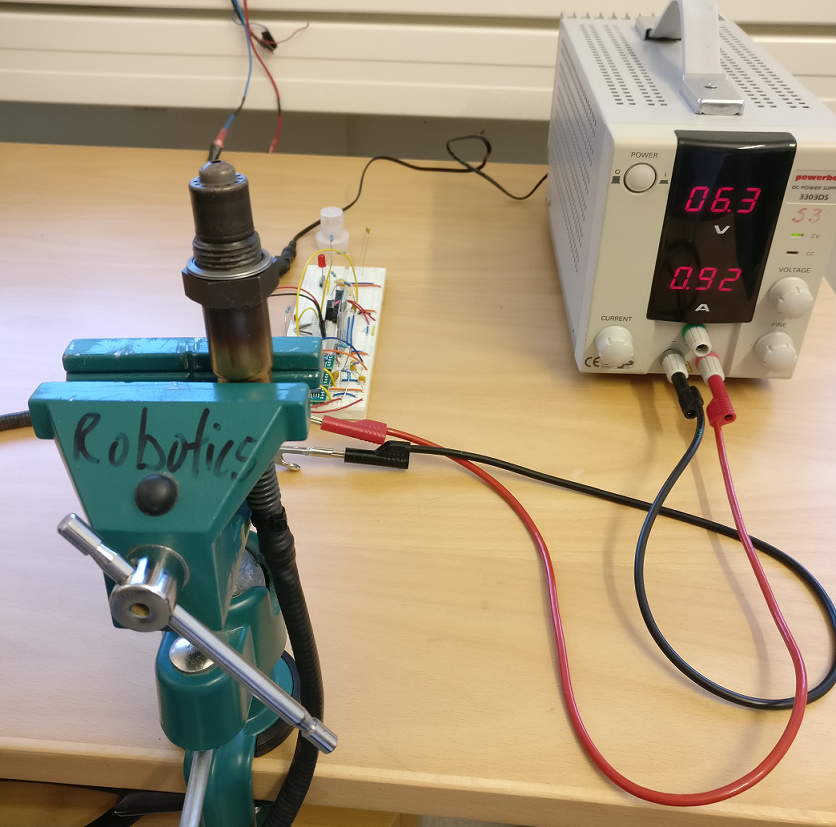
\includegraphics[width=\textwidth]{Images/lambda_bench.png}
			\end{center}
		\end{column}
%		%
%		% -----------------------------------------------
		\begin{column}{0.5\textwidth}
			\begin{itemize}
			    \visible<1->{\item Power supply for heating up sensor}
			    \visible<2->{\item Vise to avoid heating damages}
			    \visible<3->{\item 20.95 \% O$_2$ in air}
			\end{itemize}
		\end{column}	
    \end{columns}
    
    \note{ In real test no power supply is available
    
            oxygen level is also lower}
    %
\end{frame}


\begin{frame}
	%
	\frametitle{Bosch LSU4.9 Electrical Equivalent}
	\framesubtitle{Method}
	%    
	
	\begin{columns}[c] % [ b | c | t | T | onlytextwidth | totalwidth ]
		\begin{column}{0.5\textwidth}
			\begin{center}
			    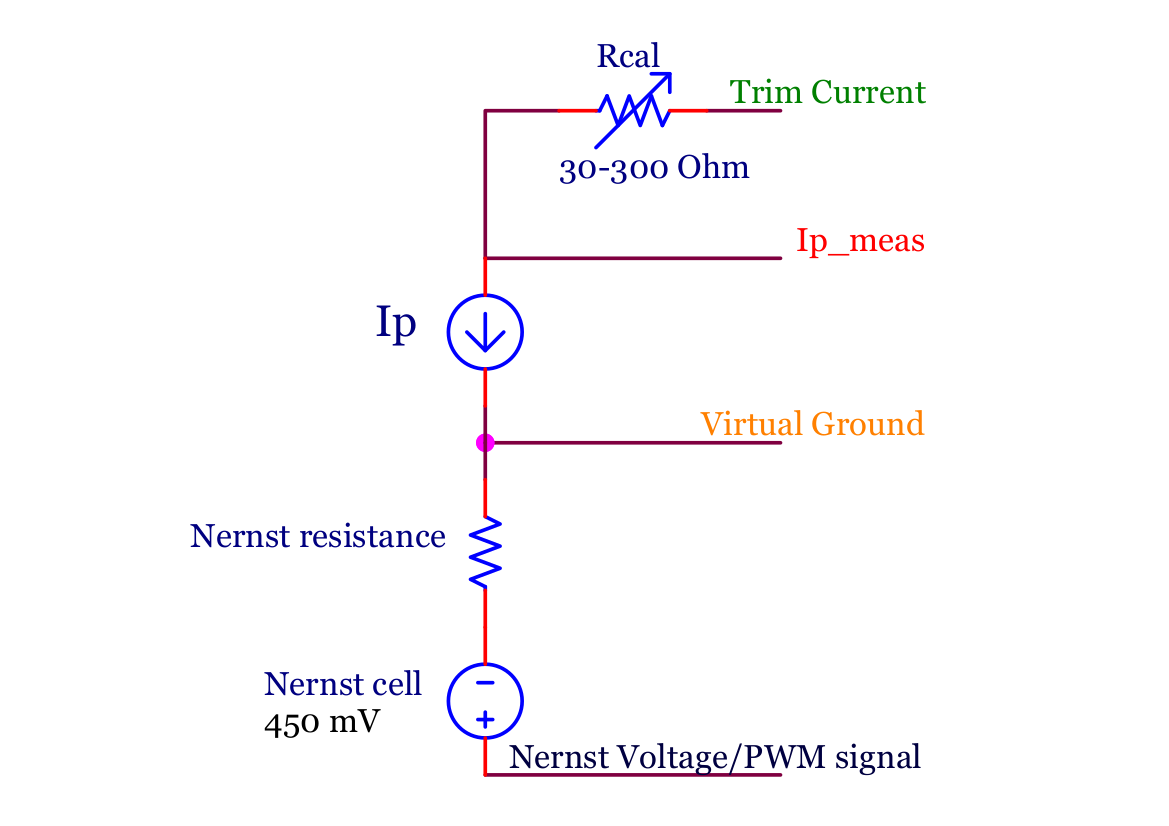
\includegraphics[width=\textwidth]{Images/SCHEMATIC1_lsu49_trans.png}
			\end{center}
		\end{column}
%		%
%		% -----------------------------------------------
		\begin{column}{0.5\textwidth}
			\begin{itemize}
			    \visible<1->{\item 4 of 6 connectors used}
			    \visible<2->{\item Rcal sensor specific}
			    \visible<3->{\item Nernst cell oxygen dependent}
			    \visible<4->{\item Nernst resistance temperature dependent}
			\end{itemize}
		\end{column}	
    \end{columns}
    
    \note{ Rcal is replaced by surface mounted resistor
    
            Ip and oxygen level can change the nernst cell voltage
            
            AC signal used to calculate the nernst resistance and also the temperature}
    %
\end{frame}



\begin{frame}
	%
	\frametitle{Prototyping on Breadboard}
	\framesubtitle{Method}
	%    
	
	\begin{columns}[c] % [ b | c | t | T | onlytextwidth | totalwidth ]
		\begin{column}{0.5\textwidth}
			\begin{center}
			    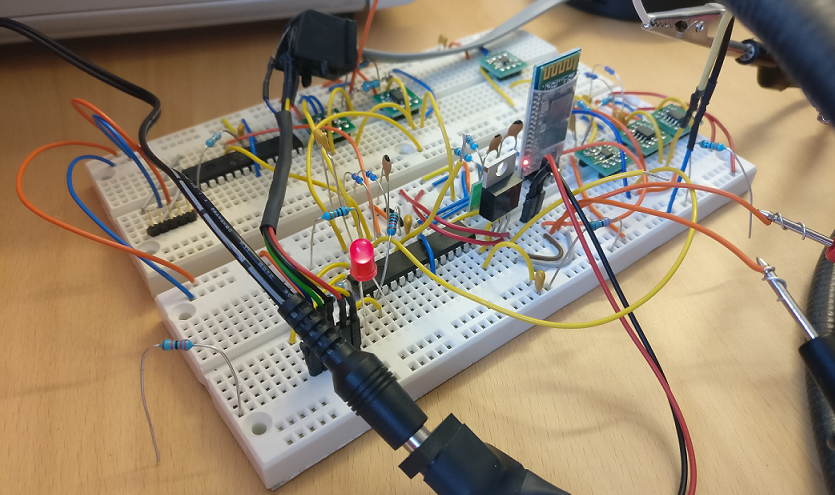
\includegraphics[width=\textwidth]{Images/breadboard.png}
			\end{center}
			\vspace{1cm}
		\end{column}
%		%
%		% -----------------------------------------------
		\begin{column}{0.5\textwidth}
			\begin{itemize}
			    \visible<1->{\item DIL package \& IC-adapters}
			    \visible<2->{\item Verify simulations}
			    \visible<3->{\item Easy to change components}
			    \visible<4->{\item Instead of using development board}
			\end{itemize}
			\vspace{1cm}
		\end{column}	
    \end{columns}
    
    \note{ PIC with DIL package
    
            Different resistor and capacitors can be tested with ease
            
            This replace the use of development board}
    %
\end{frame}



\begin{frame}
	%
	\frametitle{Schematic for MCU}
	\framesubtitle{Method}
	%    
	
	\begin{columns}[c] % [ b | c | t | T | onlytextwidth | totalwidth ]
		\begin{column}{0.65\textwidth}
			\begin{center}
			    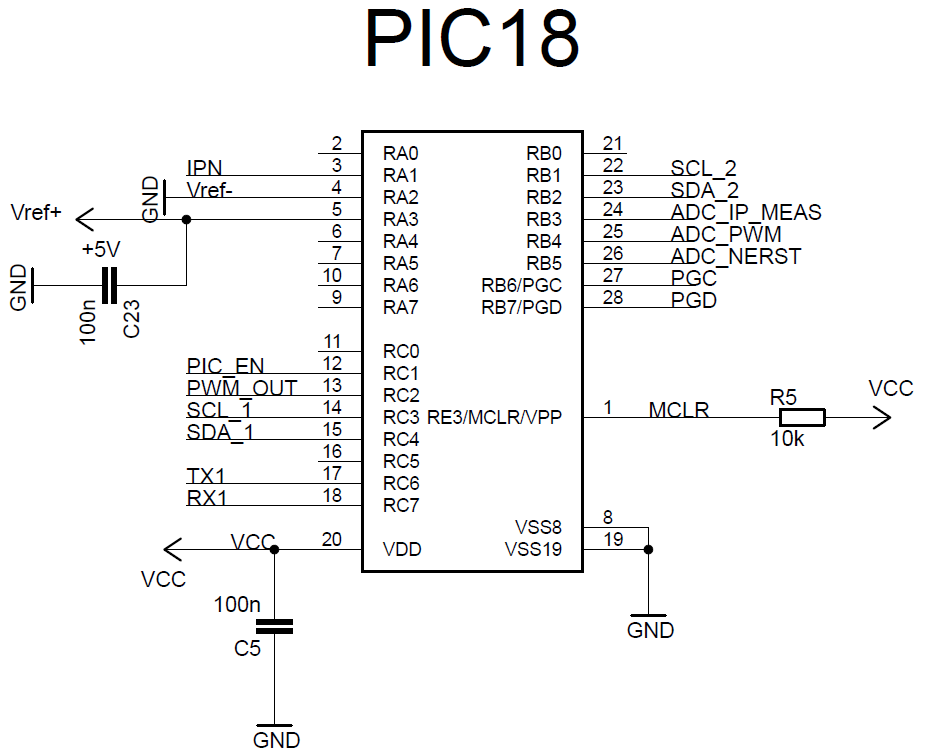
\includegraphics[width=\textwidth]{Images/PIC18_schematic.png}
			\end{center}
		\end{column}
%		%
%		% -----------------------------------------------
		\begin{column}{0.35\textwidth}
			\begin{itemize}
    			\visible<1->{\item PIC18F26K22}
			    \visible<2->{\item Two I$^2$C buses}
			    \visible<3->{\item USART for debugging}
			    \visible<4->{\item PWM for temperature}
			    \visible<5->{\item 5 ADC measurements}
			\end{itemize}
		\end{column}	
    \end{columns}
    
    \note{ I2C to Radio and DAC
    
            USART to bluetooth circuit
            
            PWM is the AC signal
            
            The ADC measurements used to calculate oxygen level and temperature}
    %
\end{frame}


\begin{frame}
	%
	\frametitle{PCB Layout}
	\framesubtitle{Method}
	%    
	
	\begin{columns}[c] % [ b | c | t | T | onlytextwidth | totalwidth ]
		\begin{column}{0.75\textwidth}
			\begin{center}
			    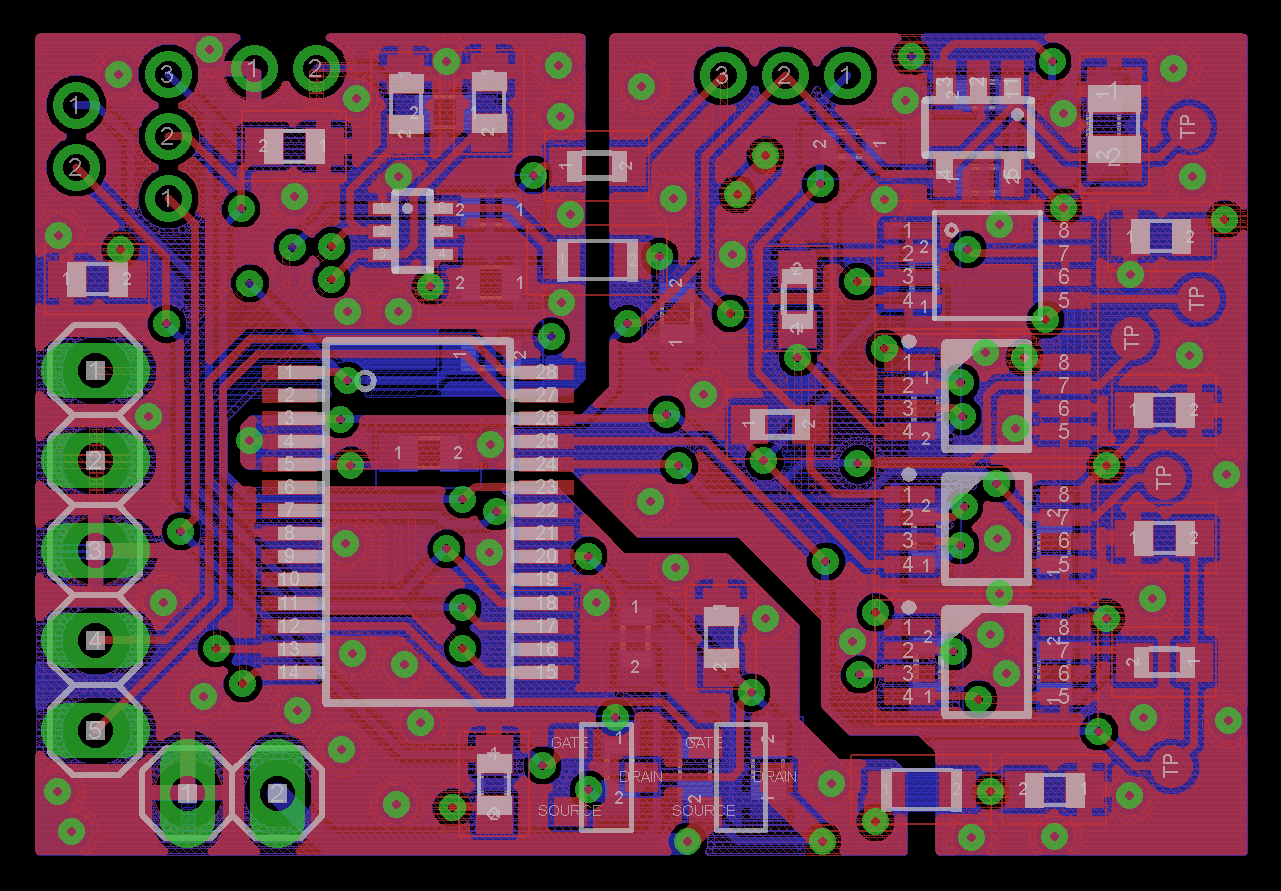
\includegraphics[width=\textwidth]{Images/PCB_layout.png}
			\end{center}
		\end{column}
%		%
%		% -----------------------------------------------
		\begin{column}{0.25\textwidth}
			\begin{itemize}
			    \visible<1->{\item Digital \& analog GND/Supply}
			    %\visible<2->{\item Two supply planes}
			    \visible<2->{\item 4 layers}
			\end{itemize}
		\end{column}	
    \end{columns}
    
    \note{ Bigger connectors on supply and programming connectors for simplicity \\
            LSU 4.9 connector too small \\
            Separate ground planes \\
            4 layer gives better possibility to place components on two sides}
    %
\end{frame}


\begin{frame}
	%
	\frametitle{Mounted PCB}
	\framesubtitle{Method}
	%    
	
	\begin{columns}[c] % [ b | c | t | T | onlytextwidth | totalwidth ]
		\begin{column}{0.65\textwidth}
			\begin{center}
			    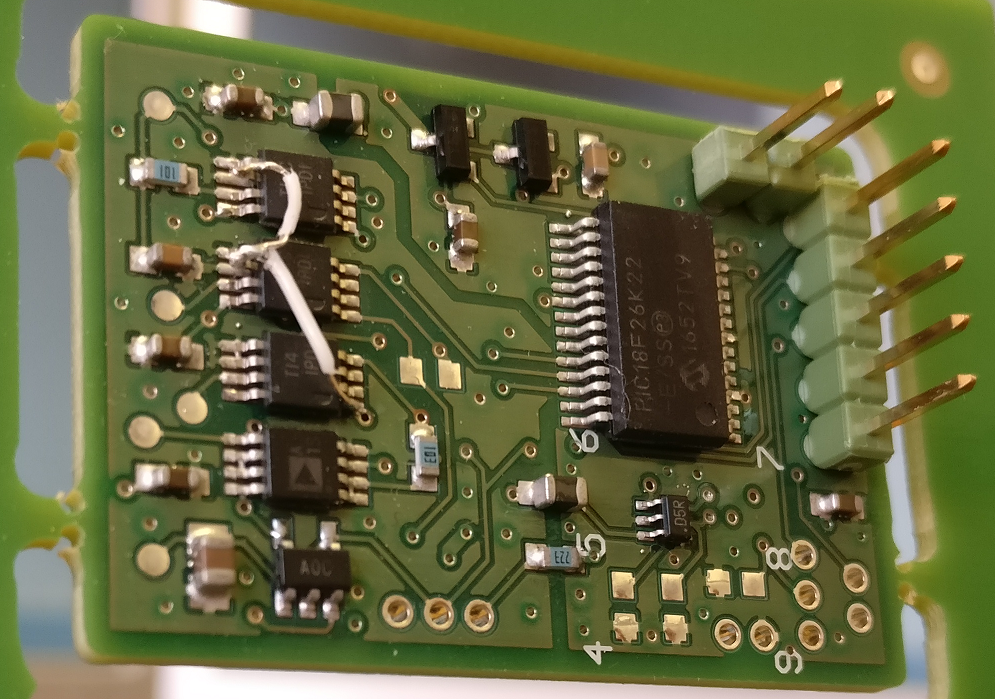
\includegraphics[width=\textwidth]{Images/PCB_monterad.png}
			\end{center}
		\end{column}
%		%
%		% -----------------------------------------------
		\begin{column}{0.35\textwidth}
			\begin{itemize}
			    \visible<1->{\item Patches with wire}
			    %\visible<2->{\item Empty positions}
			    %\visible<3->{\item PWM for temperature}
			    %\visible<4->{\item 4 ADC measurements}
			\end{itemize}
		\end{column}	
    \end{columns}
    
    \note{ Patches to set different level on reference pin
    
            Empty spots for optional components}
    %
\end{frame}


\begin{frame}
	%
	\frametitle{Software}
	\framesubtitle{Method}
	%    
	
	\begin{columns}[c] % [ b | c | t | T | onlytextwidth | totalwidth ]
		\begin{column}{0.65\textwidth}
			\begin{center}
			    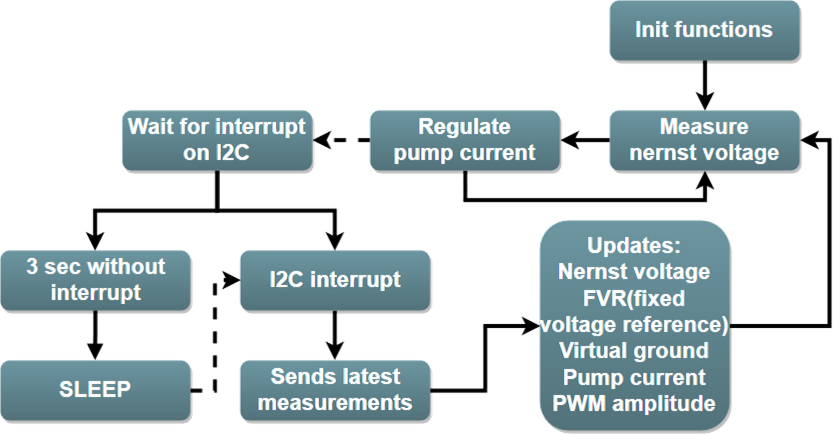
\includegraphics[width=\textwidth]{Images/Software_map_trans.png}
			\end{center}
		\end{column}
%		%
%		% -----------------------------------------------
		\begin{column}{0.35\textwidth}
			\begin{itemize}
			    \visible<1->{\item Clock speed 16 MHz}
			    \visible<2->{\item I$^2$C slave to radio unit}
			    %\visible<3->{\item PWM in 2 kHz}
			    %\visible<4->{\item 4 ADC measurements}
			\end{itemize}
		\end{column}	
    \end{columns}
    
    \note{ First initialize functions and pins, like I2C och PWM \\
            Stays in control loop for 3 seconds before entering sleep}
    %
\end{frame}



\begin{frame}
	%
	\frametitle{Electronics Before Waterproofing}
	\framesubtitle{Method}
	%    
	
	\begin{columns}[c] % [ b | c | t | T | onlytextwidth | totalwidth ]
		\begin{column}{0.65\textwidth}
			\begin{center}
			    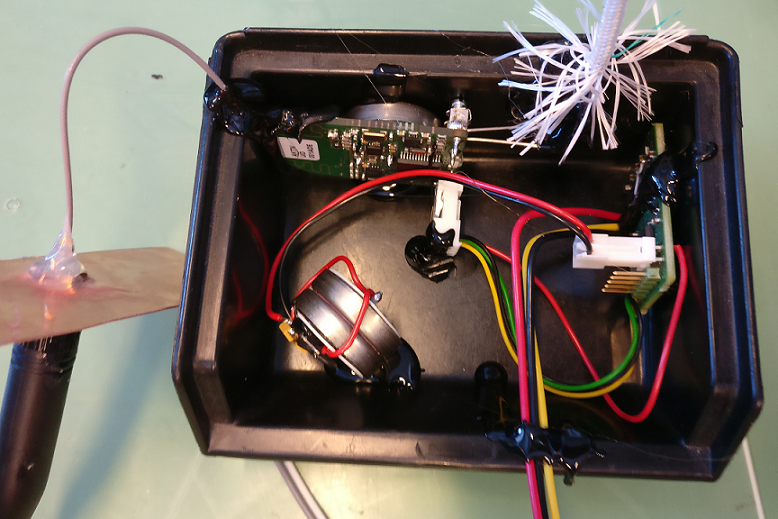
\includegraphics[width=\textwidth]{Images/electronics_box.png}
			\end{center}
		\end{column}
%		%
%		% -----------------------------------------------
		\begin{column}{0.35\textwidth}
			\begin{itemize}
			    \visible<1->{\item Antenna \& sensors goes outside}
			    \visible<2->{\item Communication wires between PCBs}
			    \visible<3->{\item Box keeps silicon in place}
			    %\visible<4->{\item 4 ADC measurements}
			\end{itemize}
			\vspace{2cm}
		\end{column}	
    \end{columns}
    
    \note{ Antenna temperature oxygen goes outside
    
            Box is filled with silicon for water proofing}
    %
\end{frame}



\begin{frame}
	%
	\frametitle{Final Mechanical Construction}
	\framesubtitle{Method}
	%    
	
	\begin{columns}[c] % [ b | c | t | T | onlytextwidth | totalwidth ]
		\begin{column}{0.5\textwidth}
			\begin{center}
			    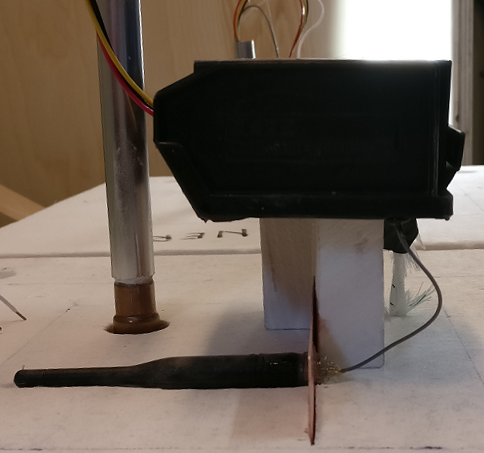
\includegraphics[height = 6.5cm]{Images/mechanical_construction_cropped.png}
			\end{center}
		\end{column}
%		%
%		% -----------------------------------------------
		\begin{column}{0.5\textwidth}
			\begin{center}
			    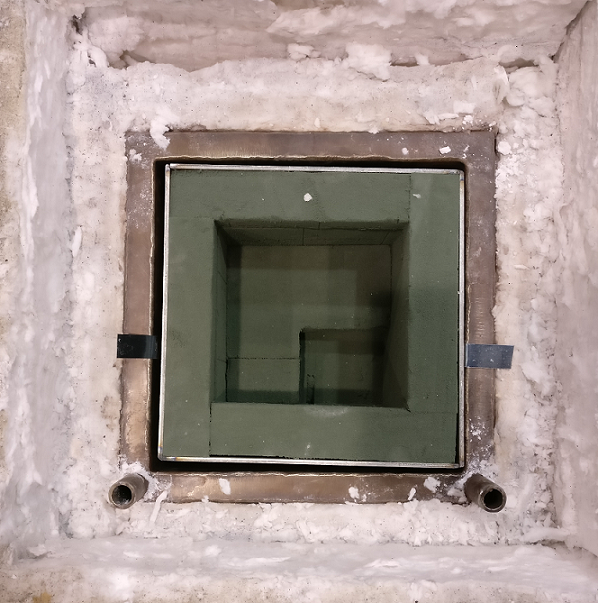
\includegraphics[height = 6.5cm]{Images/water_box.png}
			\end{center}
		\end{column}	
    \end{columns}
    
    \note{ Box to right is filled with water and flower foam
    
            Electronics inside black box and flipped into the box with water}
    %
\end{frame}



%%%%%%%%%%%%%%%%%%%%%%%%%%%%%%%%%%%%%%%%%%%%%%%%%%%%%
%                       Results                     %
%%%%%%%%%%%%%%%%%%%%%%%%%%%%%%%%%%%%%%%%%%%%%%%%%%%%%
\section{Results}

\begin{frame}
	%
	\frametitle{Table of Contents}
	\tableofcontents[subsectionstyle=hide,
	                currentsection]	% [show | shaded | hide]
	
	\note{ put your notes here }
	%
\end{frame}



\begin{frame}
	%
	\frametitle{Measurements During First Test at Mefos}
	\framesubtitle{Results}
	%
	\begin{itemize}
		%
		\visible<1->{\item{Passes from zone 1 to 3}}
		\visible<2->{\item{Averaging from LSU4.9 measurement}}
		%
	\end{itemize}
	
	%
	\vspace{0.3cm}
	%
	
	\begin{figure}
	    \centering
	    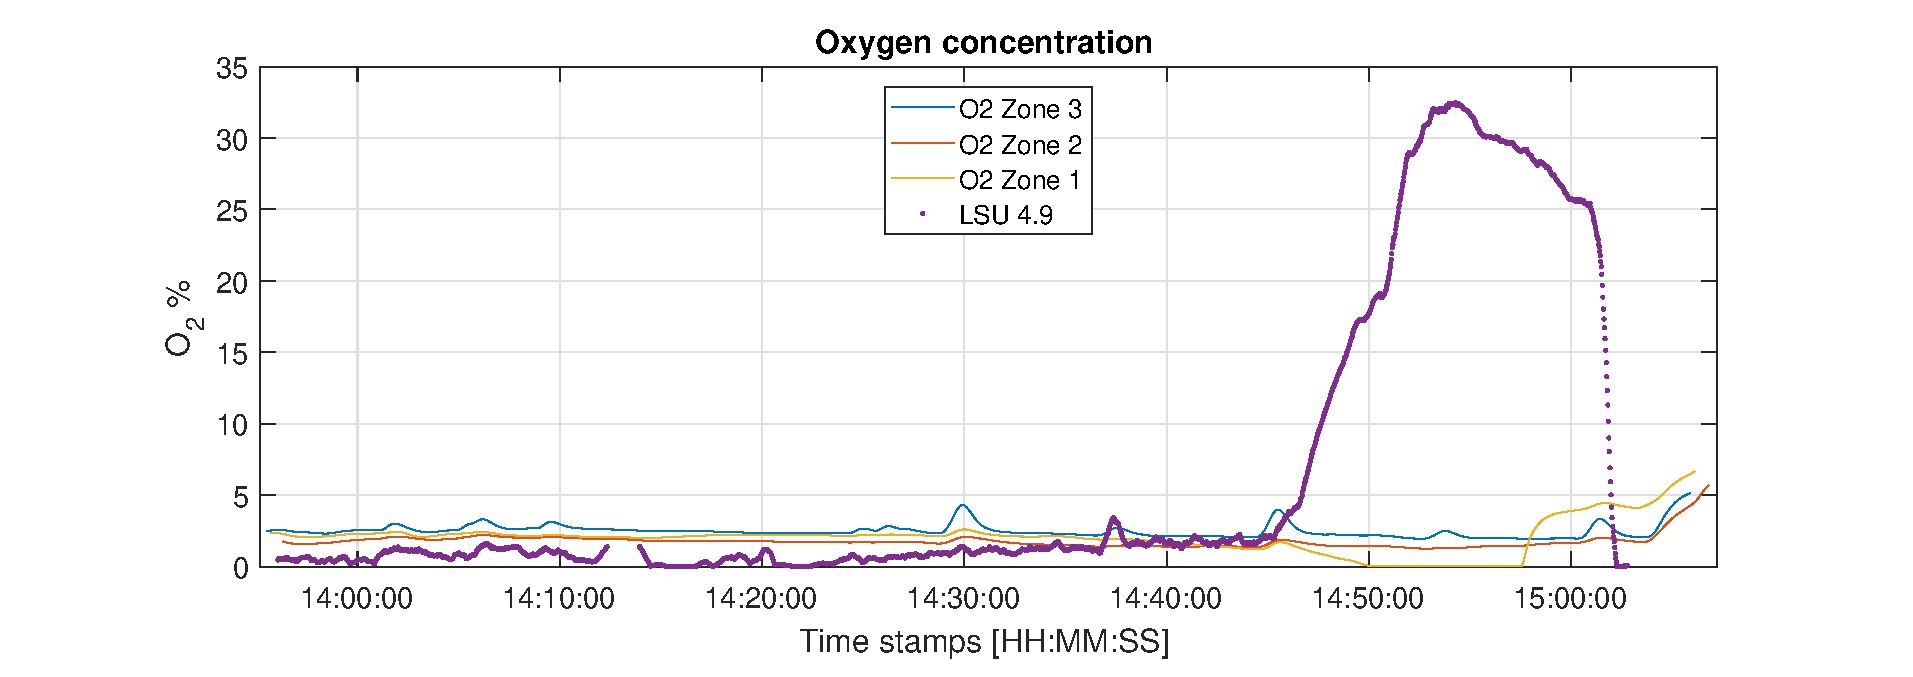
\includegraphics[width=\textwidth]{Images/syre_dots_trans.eps}
	\end{figure}
	
	\note{ Same time in the different zones
	
	        The oxygen values are averaging
	        
	        No good explanation for the peak at the end}
	%
\end{frame}



\begin{frame}
	%
	\frametitle{Measurements from a Small Oven at Mefos}
	\framesubtitle{Results}
	%
	\begin{itemize}
		%
		\visible<1->{\item{Raw values}}
		\visible<2->{\item{Compensated for temperature differences}}
		%
	\end{itemize}
	
	%
	\vspace{0.3cm}
	%
	
	\begin{figure}
	    \centering
	    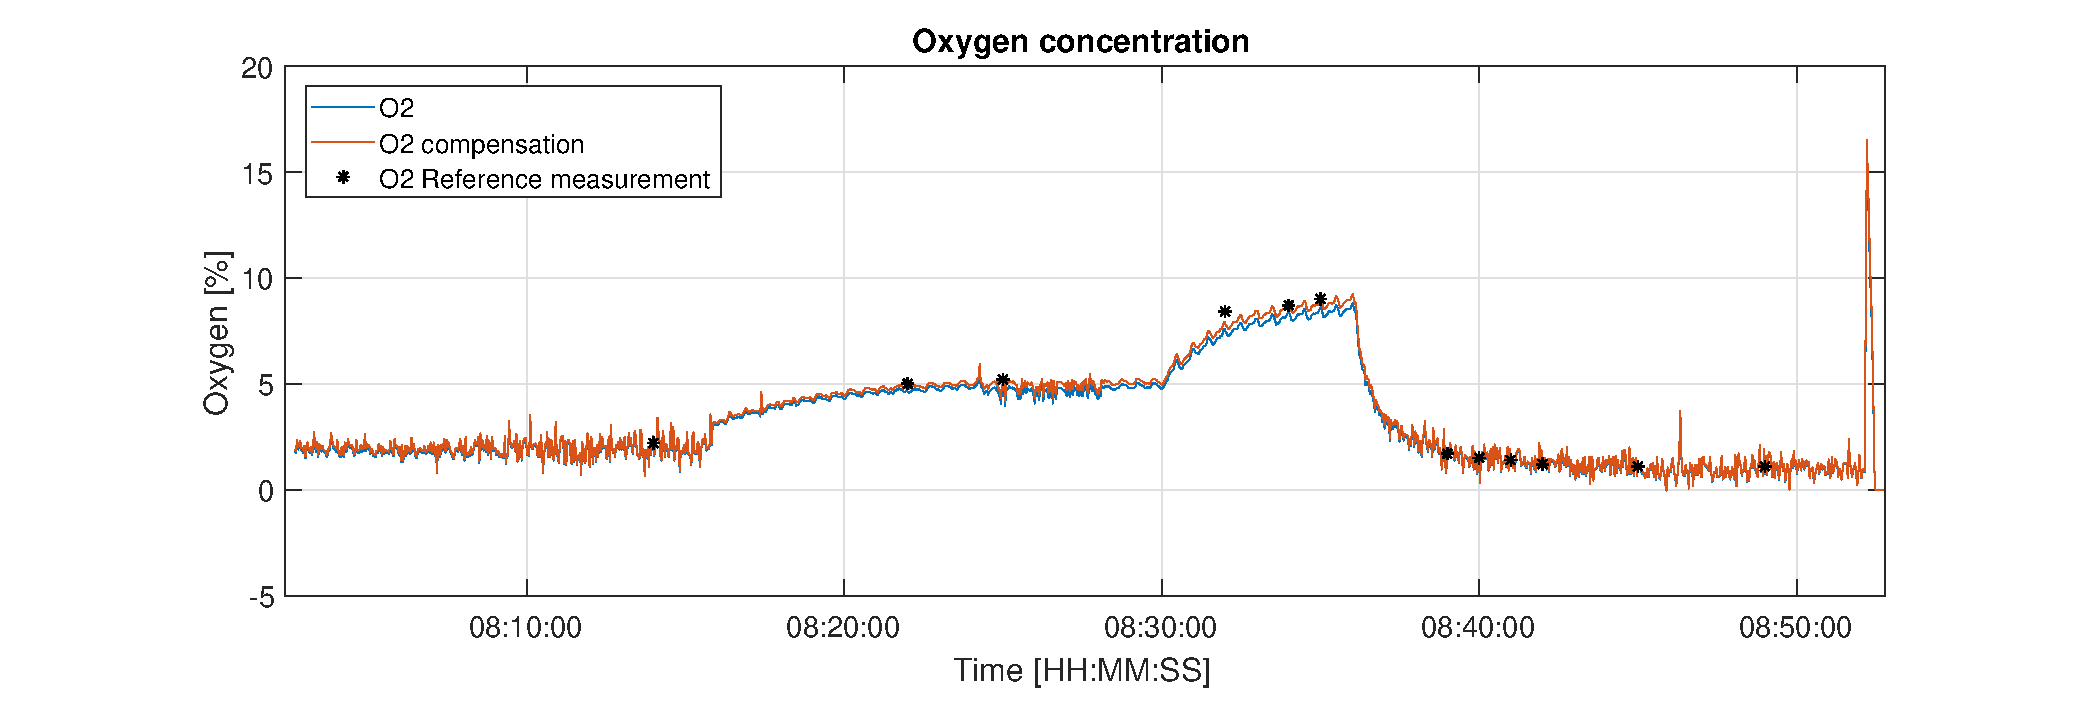
\includegraphics[width=\textwidth]{Images/oxygen_second_small_trans.eps}
	\end{figure}
	
	\note{ Done in a small oven at Mefos
	
	        Reliable values
	        
	        Referece values are logged manually}
	%
\end{frame}



%%%%%%%%%%%%%%%%%%%%%%%%%%%%%%%%%%%%%%%%%%%%%%%%%%%%%
%                   Discussion                      %
%%%%%%%%%%%%%%%%%%%%%%%%%%%%%%%%%%%%%%%%%%%%%%%%%%%%%
\section{Discussion}

\begin{frame}
	%
	\frametitle{Table of Contents}
	\tableofcontents[subsectionstyle=hide,
	                currentsection]	% [show | shaded | hide]
	
	\note{ put your notes here }
	%
\end{frame}



\begin{frame}
	%
	\frametitle{Conclusion}
	\framesubtitle{Discussion}
	%
	\begin{itemize}
		%
        \visible<1->{\item If higher robustness is achieved, the approach is good}
	    \visible<2->{\item Slow to reach operating temperature in oven}
	    %\visible<3->{\item }
	    %\visible<4->{\item 4 ADC measurements}
		%
	\end{itemize}
	
	\note{ Everything except oxygen sensor works perfect
	
	        Long time to reach correct temperature}
	%
\end{frame}



\begin{frame}
	%
	\frametitle{Future Work}
	\framesubtitle{Discussion}
	%
	\begin{itemize}
		%
        \visible<1->{\item Look into why oxygen values become unreliable after a while in the oven}
	    \visible<2->{\item Run the sensor on one cell battery (3.6 V)}
	    \visible<3->{\item Investigate the possibility to use sensor without housing}
	    %\visible<4->{\item 4 ADC measurements}
		%
	\end{itemize}
	
	\note{ Keep testing the system
	
	        One cell battery gives a smaller size and easier to integrate the system with the radio system
	        
	        The housing is big and massive. It might be good to give a more stable temperature though}
	%
\end{frame}



%\begin{frame}
%	%
%	\frametitle{Frame with two columns}
%	\framesubtitle{(subtitle)}
%	%
%	\begin{columns}[c] % [ b | c | t | T | onlytextwidth | totalwidth ]
%		%
%		% ``columns'' options usage (from the beamer user guide)
%		%
%		% [b] will cause the bottom lines of the columns to be vertically aligned.
%		% [c] will cause the columns to be centered vertically relative to each
%		%     other. Default, unless the global option t is used.
%		% [onlytextwidth] is the same as totalwidth=\textwidth.
%		% [t] will cause the first lines of the columns to be aligned. Default
%		%     if global option t is used.
%		% [T] is similar to the t option, but T aligns the tops of the first lines
%		%     while t aligns the so-called baselines of the first lines. If strange
%		%     things seem to happen in conjunction with the t option (for example
%		%     if a graphic suddenly ``drops down'' with the t option instead of
%		%     ``going up,''), try using this option instead.
%		% [totalwidth= width] will cause the columns to occupy not the whole page
%		%     width, but only width, all told.
%		%
%		% -----------------------------------------------
%		\begin{column}{0.5\textwidth}
%			column one
%		\end{column}
%		%
%		% -----------------------------------------------
%		\begin{column}{0.5\textwidth}
%			column two
%		\end{column}
%		%
%	\end{columns}
%	
%	\note{ put your notes here }
%	%
%\end{frame}





%\begin{frame}
	%%
	%\frametitle{Frame with a movie}
	%\framesubtitle{(subtitle)}
	%%
	%\movie[externalviewer]{text on the slides}{./video.wmw}
	%%
%\end{frame}


% ending page
\section*{}
\begin{frame}
	%
	\titlepage
	%
	\begin{center}
		davrag-2@student.ltu.se \\
		%david.ragnarsson@ltu.se
		%www.ee.kth.se/$\sim$XXXX/
	\end{center}
	
	\note{ put your notes here }
	%
\end{frame}



%%%%%%%%%%%%%%%%%%%%%%%%%%%%%%%%%%%%%%%%%%%%%%%%%%%%%
%                     Appendix                      %
%%%%%%%%%%%%%%%%%%%%%%%%%%%%%%%%%%%%%%%%%%%%%%%%%%%%%
\section*{Appendix}

\begin{frame}

\begin{center}
    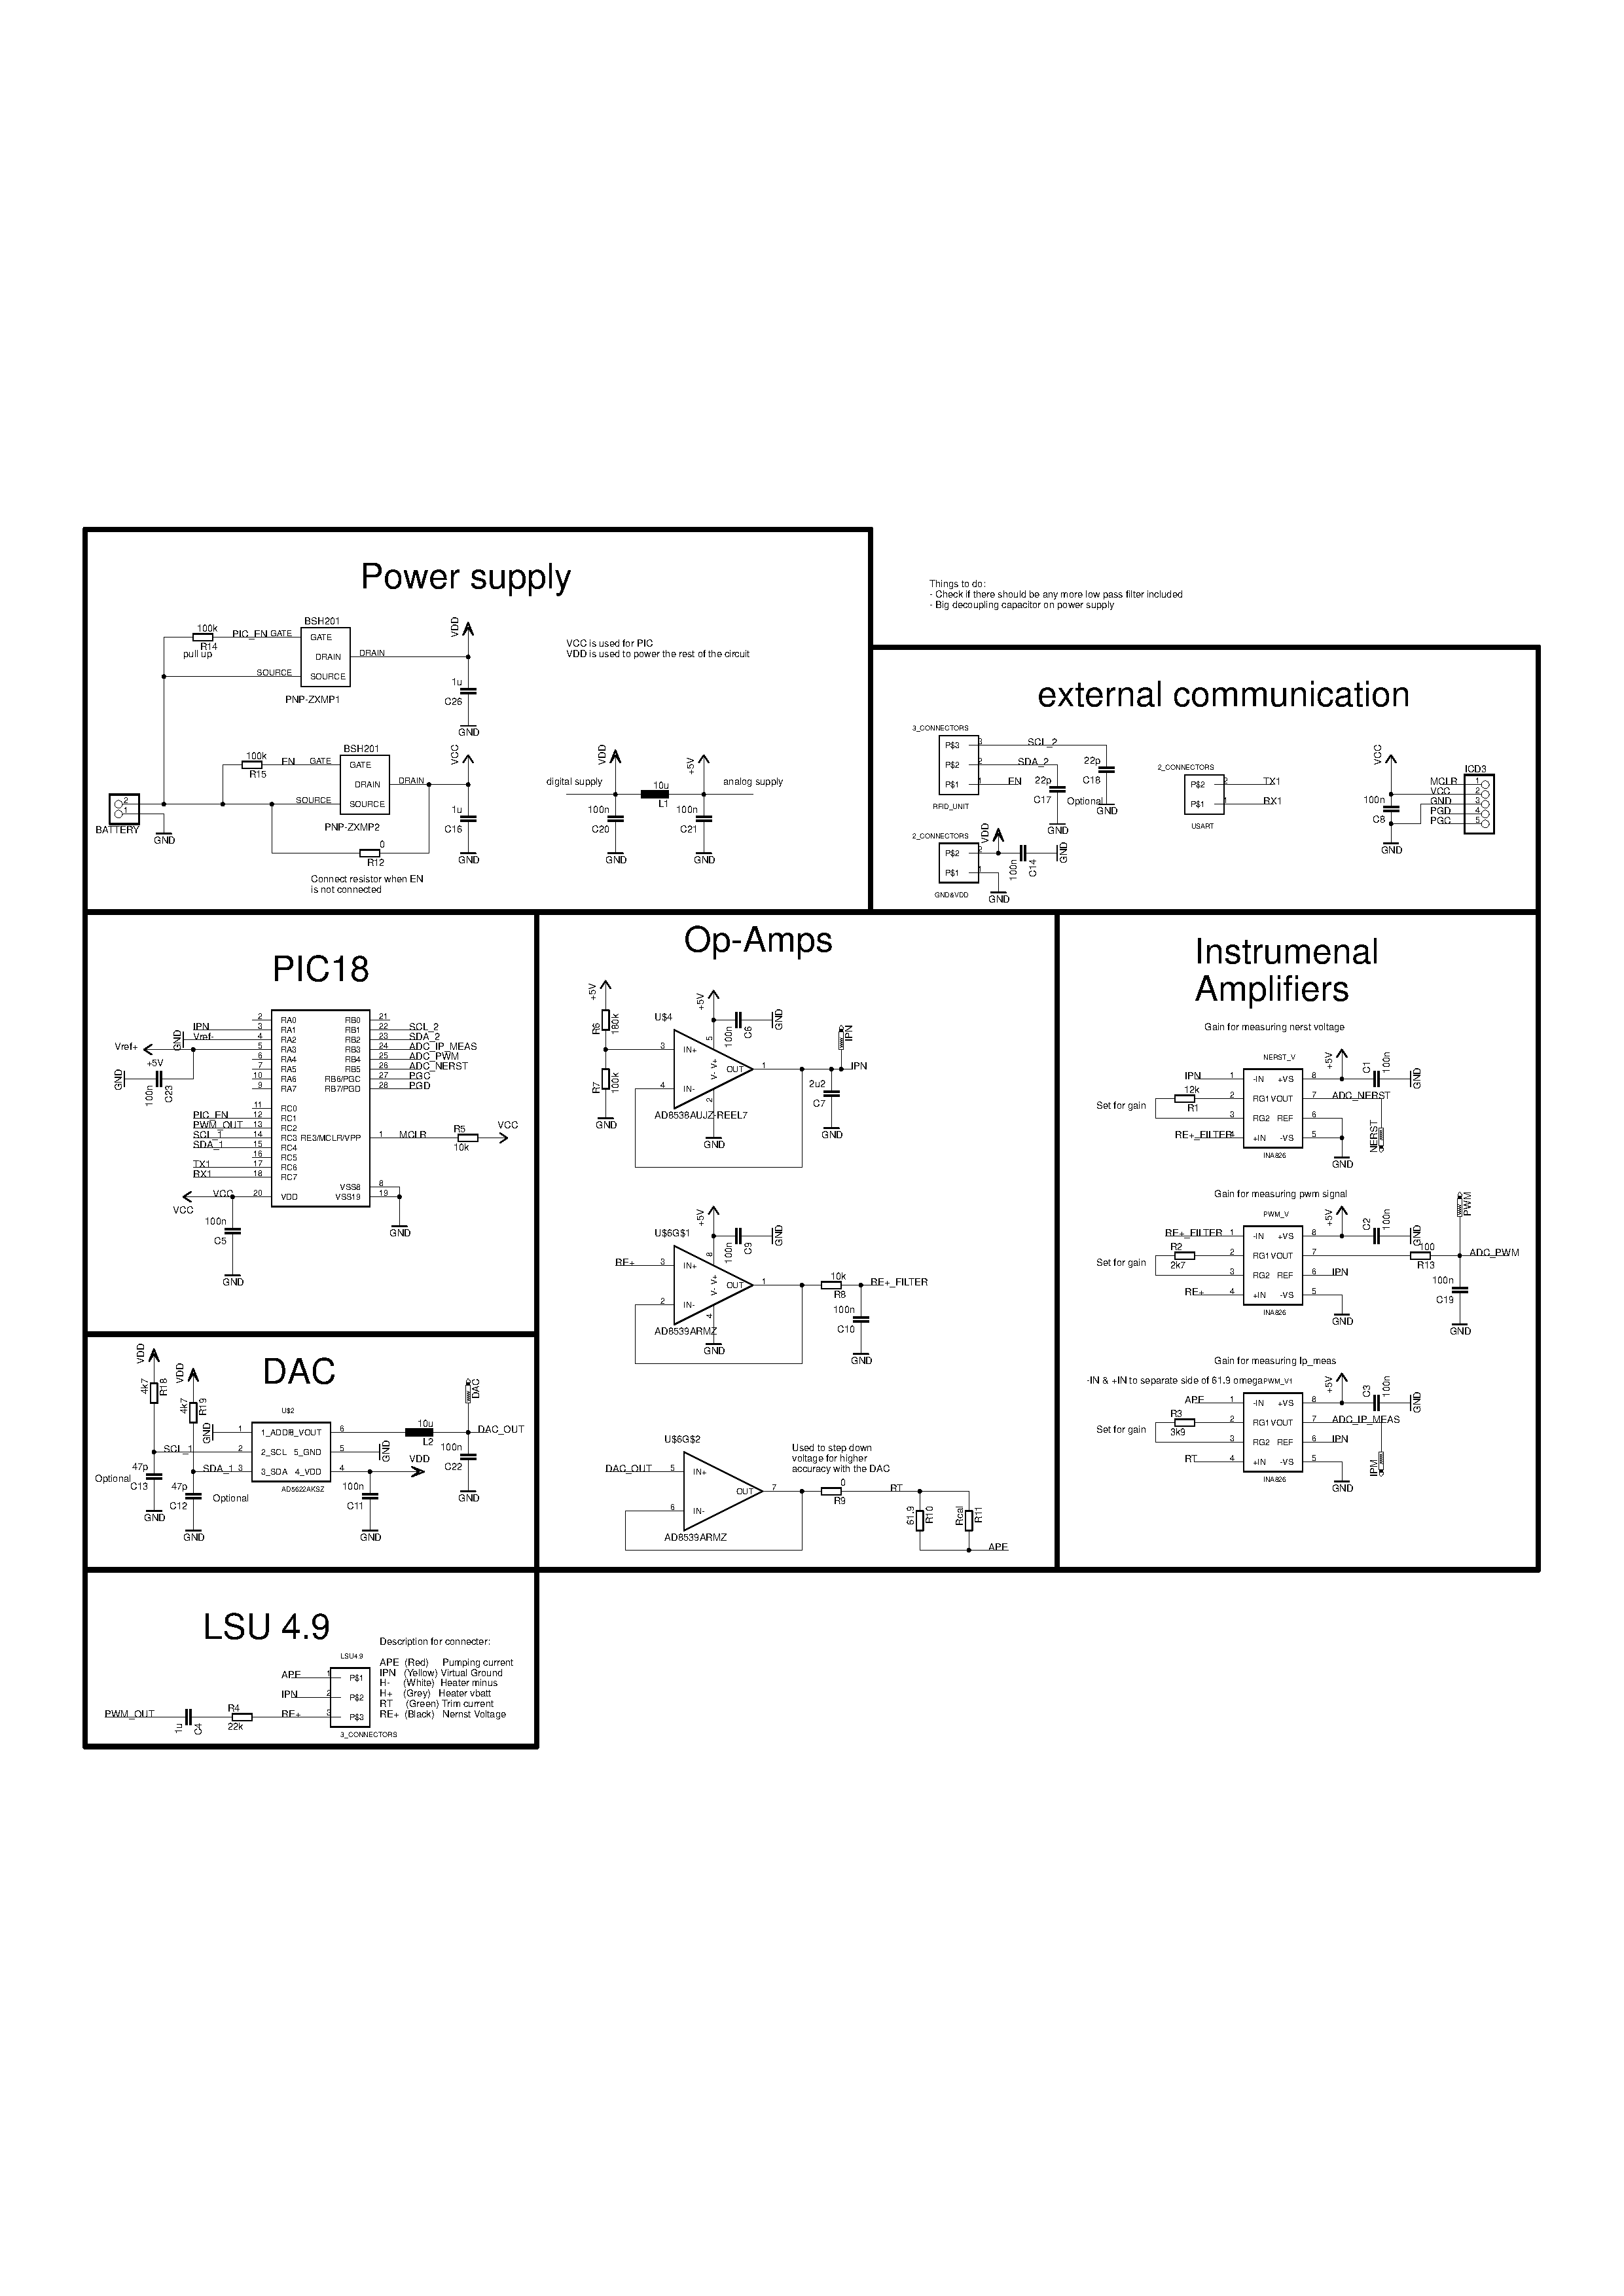
\includegraphics[width=.8\textwidth]{Images/Lambdasond_schematic.pdf}
\end{center}
    
\end{frame}


\begin{frame}

\begin{center}
    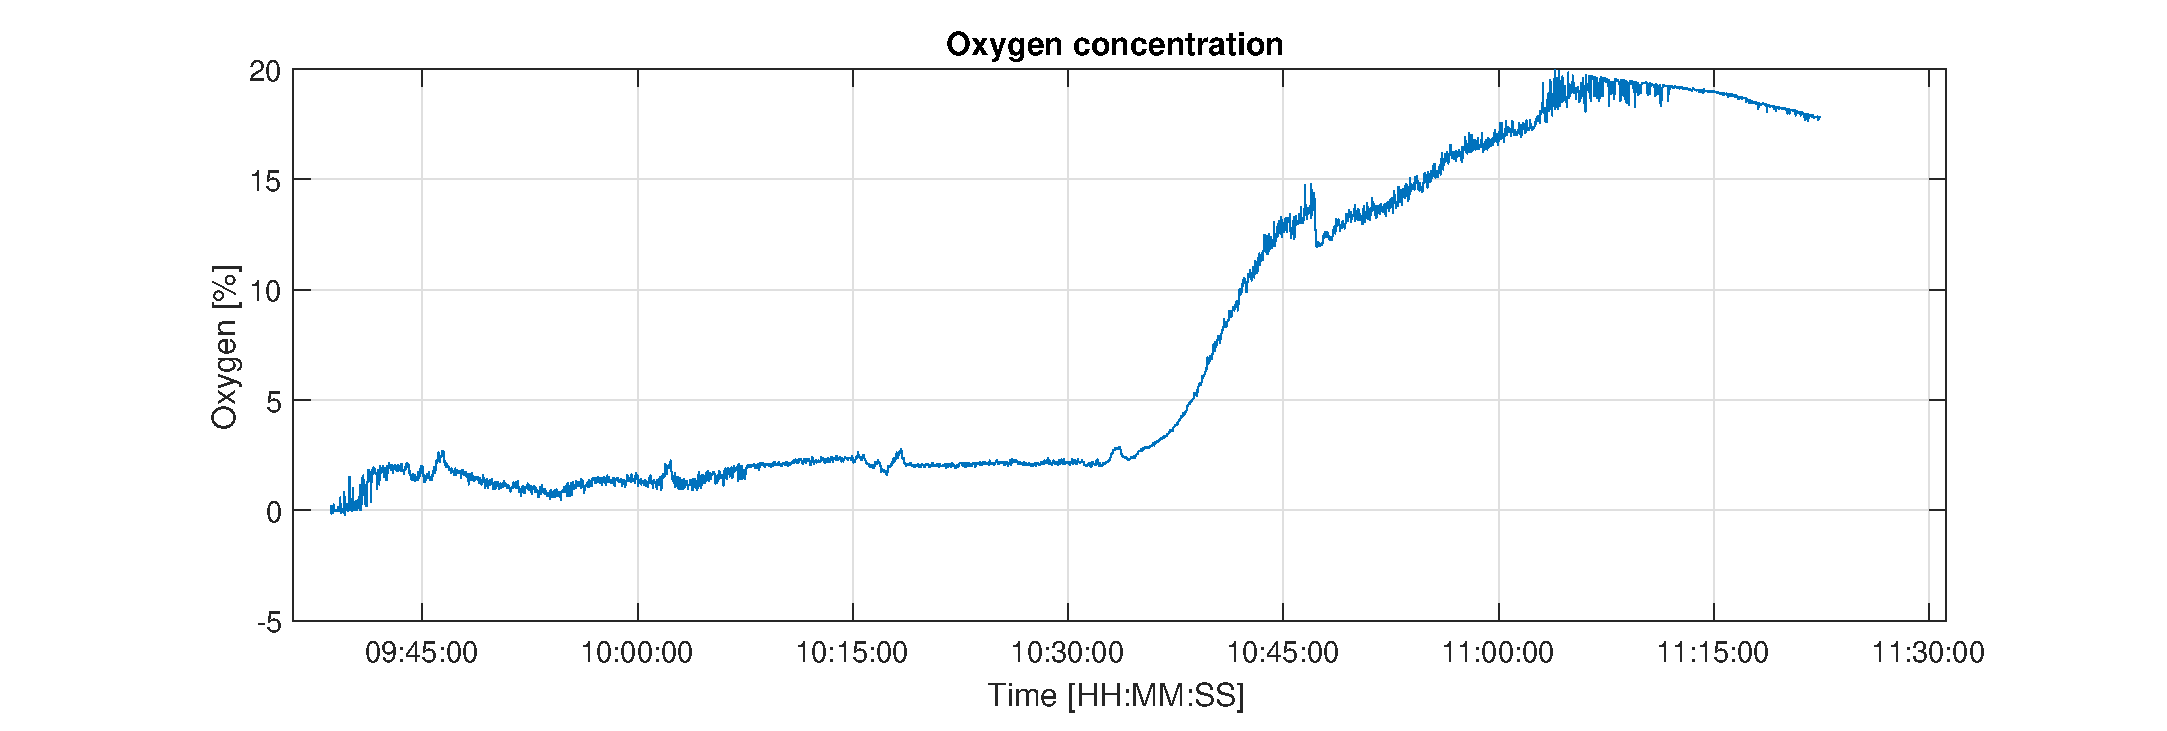
\includegraphics[width=\textwidth]{Images/oxygen_second_big.eps}
\end{center}
    
\end{frame}


\begin{frame}

\begin{center}
    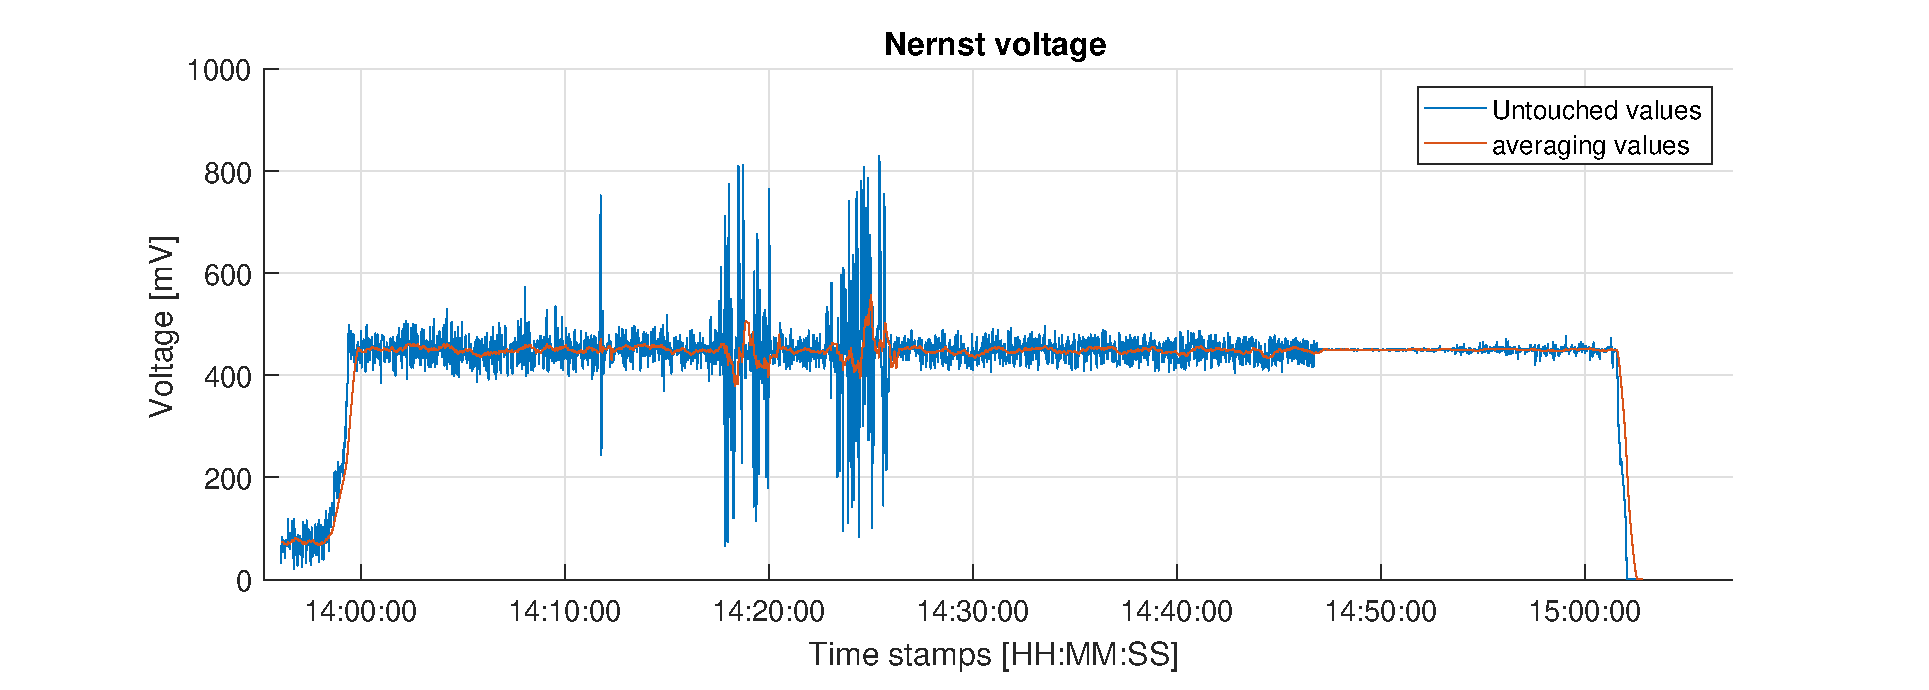
\includegraphics[width=\textwidth]{Images/nernst_both.eps}
\end{center}
    
\end{frame}


\begin{frame}

\begin{center}
    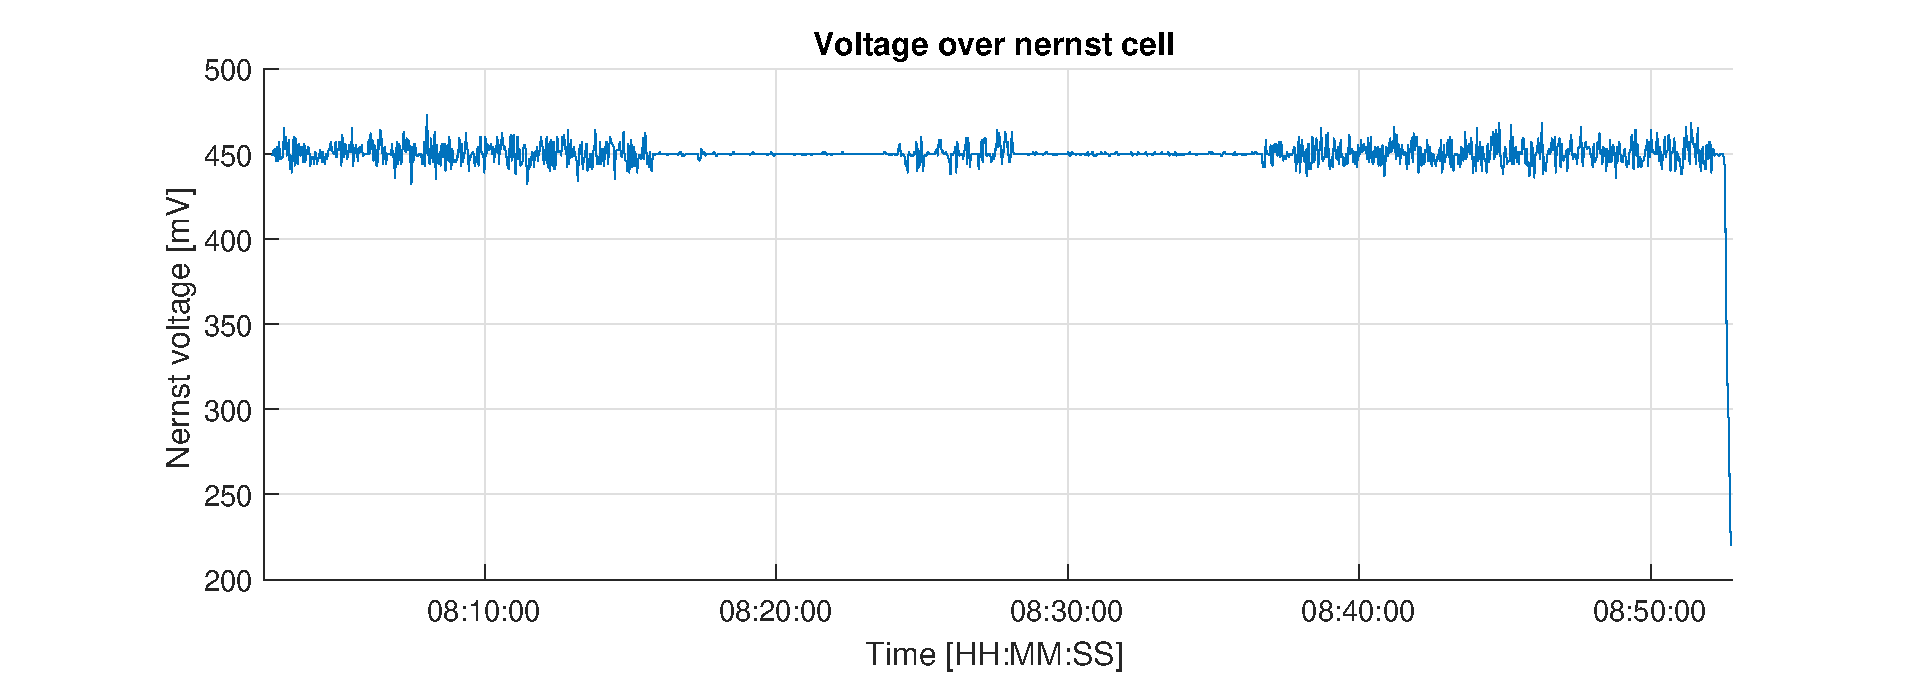
\includegraphics[width=\textwidth]{Images/nernst_second_small.eps}
\end{center}
    
\end{frame}


\begin{frame}

\begin{center}
    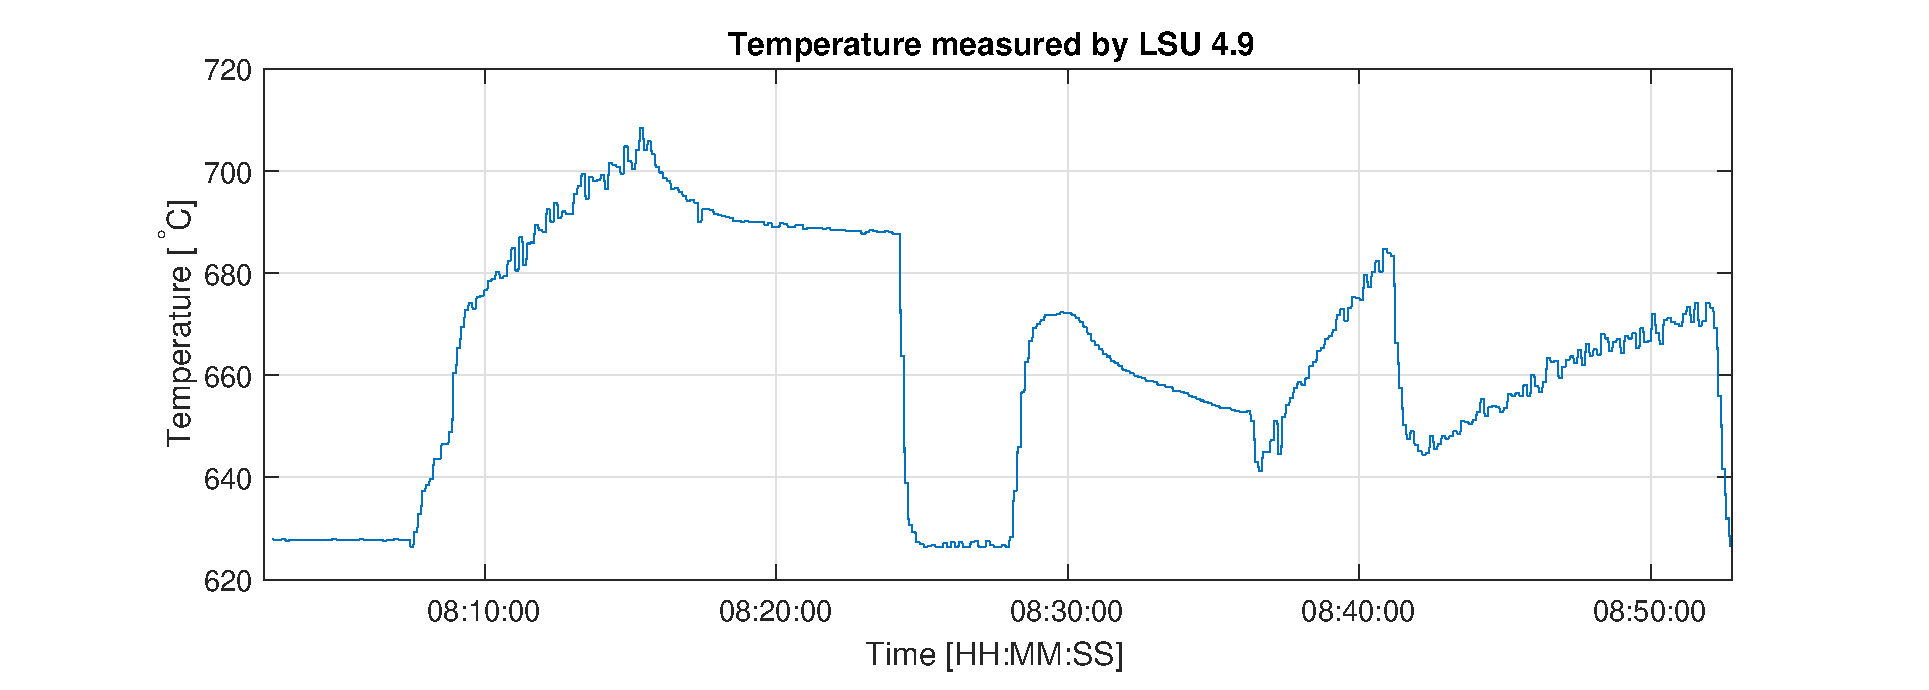
\includegraphics[width=\textwidth]{Images/temperature_second_small.eps}
\end{center}
    
\end{frame}


% bibliography
%\section*{Bibliography}
%\begin{frame}
%\begin{thebibliography}{}
%	%
%	\frametitle{Bibliography}
%	\small
%	%
%	\bibitem[1]{elements_of_style}
%	William Strunk, Jr.\ (1918)
%	\newblock The Elements of Style
%	\newblock Pearson Education Company
%	%
%	\vspace{0.3cm}
%	%
%	\bibitem[2]{promessi_sposi}
%	Alessandro Manzoni (1842)
%	\newblock I promessi sposi
%	\newblock Adelchi
%	
%	\note{ put your notes here }
%	%
%\end{thebibliography}
%\end{frame}


% ~~~~~~~~~~~~~~~~~~~~~~~~~~~~~~~~~~~~~~~~~~~~~~~~~~~~~~~~~~~~~~~~~ %
%																	%
\end{document}														%
%																	%
% ~~~~~~~~~~~~~~~~~~~~~~~~~~~~~~~~~~~~~~~~~~~~~~~~~~~~~~~~~~~~~~~~~ %
